\documentclass[a4paper,abntfigtabnum,noindentfirst]{abnt}
\usepackage[utf8]{inputenc}
\usepackage[brazil]{babel}
\usepackage{graphicx}
\usepackage[alf]{abntcite}

\begin{document}
\titulo{Resumo de ``Agile Estimating and Planning'', de Mike Cohn}
\autor{Rodrigo Soares Manhães}
\instituicao{Instituto Federal Fluminense}
\local{Campos dos Goytacazes/RJ}
\data{Março de 2010}

\maketitle
\sumario
\listoftables
\listoffigures

\chapter{The Purpose of Planning}

Plans help to guide investment decisions (this project is worth to begin?), know who needs to be available to work on a project during a given period and know if a project is on track.

Planning – especially an ongoing iterative approach for planning – is a quest for value, planning is an attempt to answer the question: ``What should we build?''

A good planning must:
\begin{itemize}

\item Reduce risk\\
Planning increases the likelihood of project success by providing insights into the project's risks

\item Reduce uncertainty\\
Iterative planning helps the team to factor knowledge about the software, for building the right software

\item Support better decision making\\
Cost and schedule estimates help to decide if start a project or not

\item Help on trade-off decisions (cost x time, functionality x effort)

\item Establish trust\\
Reliable estimates enable reliable delivery; frequent reliable delivery builds trust. Trustworthy estimates enable customers to make both prioritization and trade-off decisions

\item Convey information\\
A plan communicates and establishes a set of baseline expectations and provides confidence and verifiability for the estimates.

\end{itemize}

A good plan is one that stakeholders find sufficiently reliable that they can use it as the basis for making decisions.

Planning is an activity, not a document.

Agile planning balances the effort and investment in planning with the knowledge that we will revise the plan through the course of the project.

An agile plan is one that is easy to change.

Agile planning:
\begin{itemize}
\item is focused more on planning than the plan

\item encourages change

\item results in plans that are easily changed

\item is spread throughout the project
\end{itemize}

beautiful quote 1:
``If I were to define a failed project, one of my criteria would
certainly be `a project on which no one came up with any better ideas
than what was on the initial list of requirements.' '' (p. 6)

beautiful quote 2:
``An agile plan is one that we are not only willing but anxious to
change. We don't want to change the plan just for the sake of
changing, but we want to change because change means we've learned
something or that we've avoided a mistake.' (p. 9)


\chapter{Por que planejamentos falham}

\section{Planejamento por atividade e não por funcionalidade}

Um problema crítico com as metodologias tradicionais é que elas focam em medir o progresso do projeto por meio do acompanhamento de atividades (análise, projeto, arquitetura, testes, etc. que não agregam valor direto ao cliente) e não funcionalidades (requisitos do usuário, que são aquilo que o cliente deseja). O planejamento por atividades tem os seguintes problemas: atividades demoram a terminar, os atrasos são passados adiante no cronograma e atividades não são independentes.

\subsection{Atividades demoram a terminar (granularidade alta demais)}

Como gráficos de Gantt e similares reservam um razoável espaço de tempo para certas atividades, isto faz com que o desenvolvedor use, no mínimo, todo o tempo, mesmo que a atividade possa ser terminada em menos tempo. Muitas vezes são adicionadas funcionalidades desnecessárias ou preciosistas para cumprir o tempo restante. Em alguns ambientes, terminar antes do tempo pode até mesmo causar problemas ao desenvolvedor (acusações de estimativas altas demais, exigências por prazos menores).

\subsection{Os atrasos são passados adiante no cronograma}

Como as atividades são tipicamente dependentes entre si, atrasos se propagam no cronograma. Um atraso em qualquer uma das tarefas se traduz em atraso geral.

\subsection{Atividades não são independentes}

Atividades não são independentes e seguem uma ordem pré-estabelecida (waterfall-like), o que acumula os atrasos (2.1.2) e diminui a capacidade de responder a mudanças.


\section{Multitarefa causa mais atrasos}

A Figura \ref{efeitos-da-multitarefa} mostra que estar comprometido com duas tarefas simultaneamente aumenta um pouco a quantidade de tempo gasto com tarefas que agregam valor. Com mais de duas, este tempo útil começa a diminuir velozmente.

\begin{figure}
	\caption{Efeitos da multitarefa na produtividade}
	\label{efeitos-da-multitarefa}
	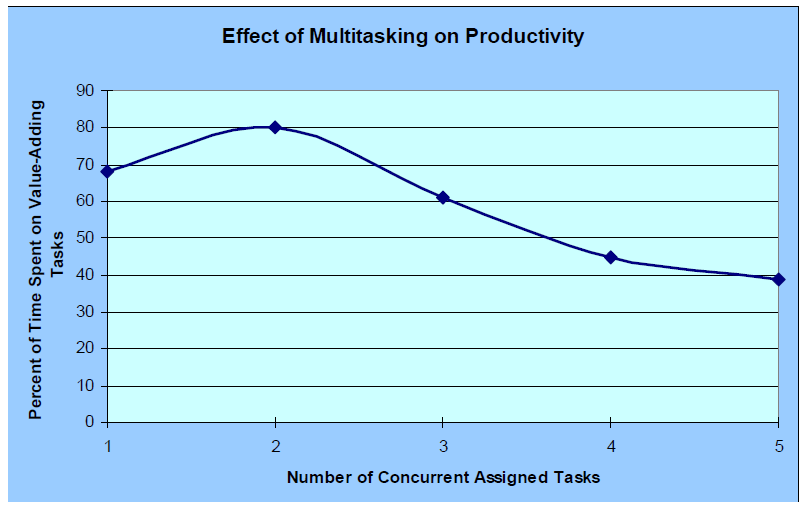
\includegraphics[scale=0.4]{efeitos-da-multitarefa}
\end{figure}

Com duas tarefas o gráfico aumenta porque quando se está emperrado em uma tarefa pode-se passar para outra. Com mais de duas o tempo de troca de contexto mental torna-se um gargalo. A multitarefa adia a data de término de cada tarefa individualmente e aumenta o work-in-progress, além de levar a um nível de trabalho mais alto do que o aconselhável, sem espaço para acomodar incertezas.


\section{Funcionalidades não são desenvolvidas por prioridade}

Planos tradicionais partem do pressuposto que TODAS as atividades previstas serão completadas. Neste contexto a priorização e a sequência de atividades são feitas de acordo com a conveniência da equipe de desenvolvimento.

Isto pode levar a que tarefas importantes para o cliente sejam deixadas para o final, podendo ter sua implementação prejudicada se ocorrer atrasos (ser implementada com qualidade baixa devido à pressa ou mesmo não ser implementada).


\section{Nós ignoramos as incertezas}

Abordagens tradicionais ignoram a incerteza, crendo que:
\begin{itemize}
\item requisitos iniciais levam a especificações completas
\item usuários não irão refinar suas opiniões nem mudar de idéia
\item não surgirão novas necessidades no período coberto pelo plano
\item é possível definir estimativas precisas para trabalho impreciso
\end{itemize}

Se um plano tentar a priori tudo que será necessário ao longo do projeto, fatalmente irá falhar.

Estimativas iniciais não devem marcar datas mas um período provável, pois o início do projeto é o período de maior incerteza. À medida que o projeto progride, as estimativas se tornam mais precisas.


\section{Estimativas tornam-se compromissos}

Toda estimativa é acompanhada, implícita ou explicitamente, de uma probabilidade de acerto. Tradicionalmente, este fato é negligenciado e estimativas são tomadas como compromissos.


\chapter{Uma Abordagem Ágil}

No Manifesto Ágil, seus autores conferem maior valor a:

\begin{itemize}
\item Indivíduos e interações do que processos e ferramentas\\
Uma equipe bem afinada com grandes profissionais e ferramentas medíocres tem melhor desempenho do que uma equipe disfuncional com profissionais medíocres e grandes ferramentas e processos A abordagem ágil busca reconhecer e trabalhar as qualidades e fraquezas individuais ao invés de tentar homogeneizar a todos

\item Software funcionando do que documentação abrangente\\
Software liberado incrementalmente e em curtos espaços de tempo torna possível obter feedback rápido, foco nas funcionalidades de maior valor e melhor satisfação do cliente.

\item Colaboração com o cliente do que negociação de contratos\\
Tradicionalmente, clientes e desenvolvedores, cuja relação é baseada em contratos de escopo fechado, estão em campos opostos; a abordagem ágil, reconhecendo que ambos têm objetivo comum (software de qualidade), procura alinhar os interesses.

\item Responder a mudanças do que seguir o plano\\
Foco principal é entregar valor ao cliente; é inevitável que os clientes tenham novas idéias ou que descartem idéias iniciais no decorrer do processo de aprendizado do software O início do projeto é o ponto de menor conhecimento. À medida que o projeto avança, mais conhecimento é adquirido e torna-se possível melhorar o plano
\end{itemize}


\section{Uma abordagem ágil a projetos}

\subsection{Uma equipe ágil trabalha como uma unidade}

Em uma equipe ágil a responsabilidade é distribuída e o time trabalha de modo coeso, não havendo subequipes (analistas, programadores, equipe de testes etc)

Papéis em uma equipe ágil:
\begin{itemize}

\item product owner
\begin{itemize}
\item assegurar-se que todos no projeto tenham uma visão unificada a respeito do projeto;
\item estabelecer prioridades de modo que a funcionalidade de maior valor seja aquela sendo trabalhada no momento;
\item tomar decisões que maximizem o ROI
\end{itemize}

quote:
``In commercial software development, the product owner is often someone from the marketing or product management side of the company. When developing software for internal use, the product owner may instead be a user, the users' manager, an analyst, or the person funding the project''

\item cliente
\begin{itemize}
\item quem financia o software
\item pode ou não ser o product owner
\end{itemize}

\item desenvolvedor
\begin{itemize}
\item qualquer um que participa do desenvolvimento do software: programadores, analistas, testadores, DBAs, designers, arquitetos, especialistas em usabilidade, redatores técnicos etc
\end{itemize}


\item gerente de projeto
\begin{itemize}
\item diferente do tradicional, foca em liderança e remoção de impedimentos ao invés de gerenciamento
\item em vários projetos, acumula outras funções como product owner ou desenvolvedor
\end{itemize}

\end{itemize}



\subsection{Uma equipe ágil trabalha em iterações curtas}

Em um projeto ágil não há fases bem definidas. Exceto algum período bem curto de modelagem e/ou projeto iniciais pregado por algumas metodologias, quando o projeto se inicia realmente, todas as atividades acontecem de modo concorrente dentro da iteração.

Iterações são timeboxed, mesmo se nem todas as funcionalidades foram terminadas. Iterações devem ser curtas. A maioria das equipes ágeis trabalha com iterações de 2 a 4 semanas. A maioria das equipes usa uma duração fixa por todo o projeto; outras definem uma duração a cada iteração.


\subsection{Uma equipe ágil entrega alguma coisa ao final de cada iteração}

A cada iteração, requisitos são transformados em software codificado, testado e potencialmente entregável. Ainda que nem toda iteração gere um release, é importante que o software esteja em um estado em que isto possa ser feito.

Como nem toda iteração gera uma entrega, foi introduzido o conceito de release, que é o resultado de um conjunto de iterações que juntas completam um conjunto de funcionalidades relacionadas. Um release tem tipicamente a duração de 2 a 6 meses.Em alguns casos o primeiro release é maior que os subsequentes.


\subsection{Uma equipe ágil tem foco em prioridades do negócio}

Uma equipe ágil entrega software na ordem estabelecida pelo product owner, de quem se espera que as priorize de modo a maximizar o ROI. Para dar flexibilidade do product owner na priorização, as funcionalidades devem ter pouca ou nenhuma dependência entre si.

Uma equipe ágil deve focar em completar tarefas que façam sentido do ponto de vista do negócio, ao invés de tarefas isoladas que só farão sentido para o cliente algum tempo depois. Uma das melhores maneiras de fazer isto é guiar-se por user stories.

Uma história é uma descrição breve de uma funcionalidade conforme vista pelo cliente ou usuário. Embora não haja uma sintaxe específica para histórias, é útil colocá-la no formato As a/I want/so that. Uma história é apenas um registro do requisito, o qual só é detalhado na iteração na qual será implementado (abordagem just-in-time).


\subsection{Uma equipe ágil inspeciona e adapta}

Um plano criado no início de um projeto não é uma garantia do que ocorrerá. Na prática, muita coisa pode mudar: pessoal pode sair, tecnologias podem trabalhar melhor ou pior que o esperado, usuários podem mudar de idéia, a concorrência pode forçar a empresa a mudar a estratégia etc. Equipes ágeis vêem a mudança como oportunidade de melhorar o plano.

Ao início de cada iteração, a equipe e o product owner procura, incorporar o conhecimento já obtido nas iterações anteriores. Se este conhecimento afeta o plano, a equipe o altera sem pestanejar de modo a melhor atender à nova visão.


\section{Uma abordagem ágil ao planejamento}

Um projeto não deve ser visto como a execução de um conjunto de passos, mas como a geração contínua de um fluxo de novas capacidades e novo conhecimento. As novas capacidades são incorporadas ao produto; o novo conhecimento possibilita fazer do produto o melhor que ele pode ser. O conhecimento gerado pode ser sobre o produto (o que o produto deve ser) ou sobre o projeto (equipe, tecnologias utilizadas, riscos). Falhas em reconhecer estes novos conhecimentos levam a estratégias que buscam conhecer tudo no início do projeto.

Na visão tradicional, se um projeto fosse uma corrida de 10 quilômetros onde a linha de chegada é conhecida e a meta é chegar a ela o mais rápido possível. Em um projeto ágil, a linha de chegada é um ponto no tempo. Neste sentido se parece mais com uma corrida baseada em tempo: chegar o mais distante possível em 60 minutos. Quando se reconhece que o resultado final é desconhecido – e mesmo impossível de ser conhecido – o planejamento se torna um processo de definição e revisão de metas que leva a um objetivo maior de longo prazo.


\subsection{Planejamento em múltiplos níveis}

É arriscado planejar para mais distante do que o horizonte visível. É preciso estabelecer marcos a partir dos quais se pode vislumbrar o novo horizonte e realizar os ajustes necessários ao plano.

A "cebola do planejamento" mostra 6 níveis decrescentes de planejamento: estratégico, portfolio, produto, release, iteração e diário.

Equipes ágeis focam, assim, em três níveis de planejamento: diário, iteração e release.

O planejamento de release considera as histórias ou temas que serão incluídos no próximo release. É feito no início do projeto, sendo atualizado no decorrer dele, normalmente ao início de cada iteração, para que reflita as expectativas atuais em relação ao que será entregue.

O planejamento da iteração é feito no início de cada iteração, baseando-se nos resultados da iteração anterior. O product owner deve priorizar as funcionalidades para a iteração dada a capacidade da equipe. Durante o planejamento da iteração são definidas as tarefas necessárias.

O planejamento diário não é um planejamento no sentido formal, mas uma rápida reunião para coordenar e sincronizar os trabalhos do dia. O foco é no planejamento das tarefas e na sincronização de atividades individuais.

As outras formas de planejamento mostradas na ``planning onion'' normalmente estão fora do escopo de uma equipe ágil.


\subsection{Condições de satisfação}

Condições de satisfação são os critérios adotados pelo product owner para medir o sucesso de um projeto.

No início do planejamento do release, a equipe e o product owner colaborativamente exploram as condições de satisfação, que normalmente incluem os itens usuais: escopo, prazo, custo e qualidade. No planejamento da iteração também são definidas as condições de satisfação para histórias individualmente. Por exemplo, para uma história “Como um usuário eu quero ser capaz de cancelar uma reserva”, as condições de satisfação poderiam ser:
\begin{itemize}
\item Um usuário que cancela uma reserva com mais de 24 horas de antecedência recebe a restituição integral do que foi pago;
\item Um usuário que cancela uma reserva com menos de 24 horas de antecedência recebe a restituição menos 25\% a título de taxa de cancelamento
\item Um código de cancelamento é mostrado no site e enviado por e-mail ao usuário
\end{itemize}

O feedback obtido ao fim de cada iteração pode ser utilizado para melhorias tanto no plano do release quanto no plano da próxima iteração.


\chapter{Estimando tamanho com story points}

Pode-se fazer uma analogia de estimativas de user stories ou funcionalidades em projetos ágeis com a expectativa que se tem a respeito do tamanho de um prato a ser servido em um restaurante: porção completa ou meia-porção de um prato; refrigerante pequeno, médio ou grande. Ou seja, estimativa por comparação. O mais importante é saber se uma funcionalidade ou story é maior ou menor que outra.

\section{Story points são relativos}

Story points são uma unidade de medida para expressar o tamanho de uma história ou funcionalidade. Ao estimar uma história, deve-se atribuir a ela um valor em pontos. O valor em si não é importante, o que importa é um valor relativo a outro. Uma história de dois pontos deve ser o dobro de uma com 1 ponto e 2/3 de uma com 3 pontos.

Não há uma fórmula para se calcular o tamanho de uma história, mas devem ser consideradas características como o esforço estimado, a complexidade do desenvolvimento, o risco e outras.

Há duas abordagens comuns para se iniciar: (1) escolhe-se aquela que se acredita ser a menor história e esta recebe o valor 1; e (2) escolhe-se uma história que se acredita ter o tamanho na média, atribuindo-se a ela um valor que esteja na média da faixa esperada de tamanhos (o autor prefere histórias entre 1 e 10 pontos). Em ambas as abordagens, as outras histórias são estimadas com base nesta primeira escolhida.

Como exemplo, imagine que tamanhos de raças de cachorros são medidos em dog points. As raças são:
\begin{itemize}
\item Labrador retriever
\item Terrier
\item Great dane (não sei o que é isso em português)
\item Poodle
\item Dachshund
\item Pastor alemão
\item São Bernardo
\item Bulldog
\end{itemize}

O labrador retriever é escolhido como o tamanho médio e lhe são atribuídos 5 pontos. Uma distribuição possível de dog points é mostrada na Tabela \ref{dog-points}.

É comum que algumas histórias não estejam completamente definidas no início da iteração, sendo o restante definido no decorrer desta. Mesmo assim estas histórias devem ser estimadas: defina algumas premissas, levante uma hipótese e vá em frente.

\begin{table}
\caption {Estimativa do tamanho de raças de cães em dog points}
\label{dog-points}
\begin{center}
\begin{tabular}{| r | l |}
\hline
Labrador Retriever & 5\\
\hline
Terrier &3\\
\hline
Great dane & 10\\
\hline
Poodle & 3\\
\hline
Dachshund & 1\\
\hline
Pastor alemão & 5\\
\hline
São bernardo & 9\\
\hline
Bulldog & 3\\
\hline
\end{tabular}
\end{center}
\end{table}


\section{Velocidade}

Velocidade é a medida da taxa de progresso de uma equipe, consistindo na soma do número de story points atribuídos a cada história completada na iteração. Se a equipe completou 3 histórias de 5 pontos na última iteração, a velocidade da equipe é de 15.

Se uma equipe completou 10 story points na última iteração, podemos acreditar que ela completará 10 story points na iteração atual (a idéia de yesterday weather do XP).

Se forem somadas as estimativas em story points de todas as funcionalidades desejadas, teremos a estimativa do tamanho total do projeto. Se a velocidade da equipe é conhecida, podemos dividir o tamanho do projeto pela velocidade e estimar o número de iterações e, consequentemente, uma duração para o projeto.

Esta explicação de planejamento de releases é bastante simplista mas funcionará por enquanto (o livro traz, mais a frente, maiores detalhes a este respeito)


\subsection{A velocidade corrige erros de estimativa}

A beleza desta abordagem é que a aplicação do conceito de velocidade auto-corrige erros de estimativa. Suponha que um projeto é estimado para 200 pontos e o time acredita que sua velocidade é de 25 pontos por iteração, o que significa que a duração estimada é de 8 iterações. Contudo, uma vez que o projeto se inicia, verifica-se que a velocidade da equipe é de 20 pontos. Sem fazer nenhuma reestimativa, pode-se identificar que com esta velocidade o projeto terá então 10 iterações em lugar de 8.

A estimativa por pontos tem a boa característica de separar completamente a estimativa de esforço da estimativa de duração. Evidentemente, esforço e duração são relacionados, mas separá-los permite que possam ser pensados separadamente. Note que a duração do projeto não é estimada, mas calculada. A distinção é sutil, mas importante.



\chapter{Estimando em dias ideais}

Se nos perguntarmos quanto tempo dura um jogo de futebol, há duas respostas possíveis:
\begin{itemize}
\item dois tempos de 45 minutos, ou seja, 90 minutos, 1 hora e meia;
\item cerca de 2 horas, se contarmos 15 minutos de intervalo e os eventuais acréscimos aos dois tempos.
\end{itemize}

A diferença está no modo de medir. A primeira é o tempo ideal, medido levando-se em conta apenas o tempo regulamentar e nada mais. A segunda é o tempo decorrido, que leva em conta o tempo conforme contado no relógio. Cada forma de medir serve a um propósito: a primeira, para os árbitros, geração de estatísticas e demais questões técnicas; a segunda, para a grade de programação das emissoras e para o público.

Normalmente, é bem mais fácil estimar por tempo ideal, pois não é necessário levar em conta a complexidade e as incertezas do mundo real.

Ainda na analogia do futebol, imagine que um jogo transmitido pela televisão, e na programação foi atribuído um tempo de 2 horas para a transmissão. Este tempo é evidentemente uma estimativa. Se houver, por exemplo, uma briga generalizada entre os dois times no meio da partida o jogo atrasará e, digamos que o tempo decorrido entre o início e o fim do jogo seja de 2 horas e 20 minutos. A parte do público da TV que deseja assistir ao programa após o futebol terá seu entretenimento atrasado. Podem ficar chateadas ou aborrecidas com isto, mas nunca surpresas, pois a duração do jogo de futebol é uma estimativa. Do mesmo modo, não é de surpreender quando um projeto de software estimado para 12 semanas gasta, por exemplo, 13.

\section{Tempo ideal e desenvolvimento de software}

Em um projeto de software, o tempo ideal difere do tempo decorrido devido ao overhead natural do dia-a-dia. Além da história corrente, um desenvolvedor típico eventualmente gasta tempo com outras coisas tais como suporte e manutenção dos releases em produção, reuniões, apresentações, questões pessoais, telefone, estudo e treinamento, e-mail, alternância entre tarefas, pequenas questões administrativas etc.

É comum um gerente perguntar a um desenvolvedor quanto tempo uma determinada tarefa irá levar e o desenvolvedor responder ``Cinco dias'', o que o gerente toma como um compromisso. Porém, a realidade, muitas vezes não percebida claramente, é: ``Cinco dias se eu fizer apenas isso. Como faço outras coisas, provavelmente ficará pronto em 2 semanas''.

Para o cálculo dos dias ideais, assume-se que:
\begin{itemize}
\item a história sendo estimada é a única coisa com a qual o desenvolvedor irá se ocupar;
\item tudo o que o desenvolvedor necessitar estará à mão quando ele começar;
\item não haverá interrupções.
\end{itemize}


\section{Dias ideais como uma métrica de tamanho}

Ao estimar por dias ideais, não é necessário levar em consideração todo o eventual overhead. Dependendo do ambiente e da cultura da organização, a diferença entre dias ideais e dias decorridos poderá ser maior ou menor.

Quando não se levando em conta o overhead do mundo real, dias ideais são uma estimativa de tamanho, exatamente como os story points. Também como estes, um tamanho expresso em dias ideais pode ser utilizado para se obter uma estimativa de duração do projeto usando a velocidade.


\section{Uma estimativa, não muitas}

Quando se escolhe estimar por dias ideais, apenas uma estimativa deve ser agregada a cada história. Algumas equipes estimam histórias por papel: x dias ideais para o programador, y dias ideais para o DBA, z dias ideais para o webdesigner e por aí vai. Na imensa maioria dos casos, isto não é aconselhável, pois remove o foco na idéia de ``estamos todos juntos nisto'' que agile traz. Além disto, a adoção desta estratégia complica bastante o planejamento dos releases e das iterações, além de gerar uma velocidade para cada papel. O autor, por outro lado, cita um caso onde isto foi justificado: uma equipe teria que gerar três versões funcionalmente idênticas de um produto, para Windows, MacOS e handhelds. Como os indivíduos não tinham condições técnicas de atuar em mais de uma frente destas três, optou-se por estimar separadamente os tamanhos em dias ideais.



\chapter{Técnicas de estimativa}

Nem sempre dedicar o máximo esforço possível a uma determinada tarefa é a melhor coisa a fazer. Muitas vezes, por apenas uma fração deste esforço é possível obter resultados adequados. Isto vale para o esforço despendido em estimativas. Para o autor, a curva precisão da estimativa (eixo y) por esforço é como uma parábola, ou seja, ele argumenta que há uma certa quantidade de esforço até a qual a qualidade das estimativas é crescente. Desta quantidade de esforço em diante, a precisão da estimativa passa a decair. Além disto, mesmo o ponto máximo da parábola não chega a 100\% de precisão, talvez nem a 80\%.

A ilusão da previsibilidade é uma armadilha para muitos projetos, que visando obter uma estimativa de máxima precisão realiza uma grande quantidade de trabalho up-front e ainda assim as estimativas não são as desejadas.

Uma equipe ágil prefere ficar na metade crescente da parábola, reconhecendo que é impossível eliminar a incerteza e buscando a dose correta onde pequenos esforços trazem grandes resultados (p. ex. a regra 20-80). Mesmo recusando um grande esforço de planejamento, planos ágeis tendem a ser mais confiáveis no decorrer do tempo, pois são norteados por entrega de frequente de pequenos incrementos código completamente funcional, testado e integrado

\section{Estimativas são compartilhadas}

Equipes ágeis estimam em grupo, por todos os membros, pois normalmente não se sabe a priori quem será responsável pela implementação de nenhuma história em particular. Além disto, a diversidade de opiniões tende a minimizar vícios individuais, tanto de demasiado otimismo quanto de pessimismo.


\section{A escala de estimativa}

Nós somos melhores em estimar coisas dentro de 1 ordem de magnitude. Assim, estimativas ágeis são feitas dentro de uma faixa. O autor tem tido sucesso com duas escalas:
\begin{itemize}
\item 1, 2, 3, 5 e 8 (fibonacci);
\item 1, 2, 4 e 8 (dobro)
\end{itemize}

Embora ambas funcionem bem, o autor tem ligeira preferência pela primeira. Tomando esta como base, caso uma história seja vista como um pouco maior que outra à qual foi atribuído 5, não há problemas em atribuí-la 5 também. Por outro lado, uma história que mereceria um 7 poderia perfeitamente ser aproximada para 8.

É útil permitir que zero seja um valor válido para estimativas. Como as estimativas são relativas e estamos em uma escala de 8x, definir 1 para histórias minúsculas pode limitar muito o tamanho máximo das histórias. Além disto, se uma história é muito mais próxima de zero que de 1, atribuir 1 poderia trazer ruído ao cálculo da velocidade.

Se a equipe adota zero na escala, é preciso fazer todos na equipe (principalmente o product owner) entender que 15 vezes zero não é igual a zero. Uma história de zero pontos pode ser vista como gratuita, mas 10 delas não. Uma alternativa o uso de zero é definir uma estimativa única para um grupo de histórias minúsculas.

Algumas equipes preferem valores como 10, 20, 30, 50 e 100. Não há problema, pois estão todos na mesma ordem de magnitude. Contudo deve-se estabelecer, assim como com números pequenos, os valores aceitáveis. Não se pode permitir uma história estimada como 66 e outra como 67, pois é um nível de precisão falso, já que não é possível discernir a 1\%.


\section{Histórias, épicos e temas}

Embora sempre seja preferível estimar histórias cujos tamanhos sejam pequenos, nem sempre isto é possível, pois nem todos os requisitos se apresentam em uma granularidade tão fina. Estimativas iniciais, por exemplo, para requisitos de alto nível que não serão implementados no futuro próximo, por exemplo. Ou quando se está analisando a viabilidade de se implementar um módulo. Para estes casos, é desejável ter uma grande história, que normalmente é chamda de épico.

Além disto, um conjunto de histórias relacionadas pode ser combinada e tratada, para fins de estimativa ou planejamento de release, como um todo. Este conjunto normalmente é chamado de tema.

É necessário sempre ter em mente que estimativas para épicos ou temas sempre terão um grau de incerteza muito maior do que estimativas para histórias comuns.

Histórias que serão abordadas em um futuro próximo (ou seja, nas próximas iterações) precisam ser pequenas o suficiente para caber em uma iteração, devendo ser estimadas com números pequenos (1, 2, 3, 5, 8, por exemplo). Histórias cuja implementação está mais distante podem ser mantidas como épicos. O autor utiliza os valores de 13, 20, 40 e 100 para estes casos.


\section{Derivando uma estimativa}

As técnicas mais comuns (que podem ser usadas isoladamente ou em conjunto) são:
\begin{itemize}
\item opinião de especialista
\item analogia
\item desagregação
\end{itemize}

\subsection{Opinião de especialista}

Esta abordagem é simplesmente perguntar a alguém que conheça bem o assunto em questão. Isto é mais útil em histórias que não envolvem conhecimentos que não possam ser dominados por uma só pessoa. Embora seja baseada em intuição, há evidências que dizem que este tipo de abordagem costuma ser mais precisa do que abordagens mais analíticas (Phillip Johnson et al., Empirically Guided Software Effort Estimation. IEEE Software, 17(6), pp. 51-56, 2000).

\subsection{Analogia}

Nesta abordagem, uma história é estimada comparativamente a outras. Uma técnica útil é a triangulação: uma história estimada como 5 deve ser maior que uma estimada como 3 e menor que uma de 8. Há evidências de que estimamos melhor usando comparações do que tamanhos absolutos.

\subsection{Desagregação}

Na desagregação, uma história é dividida em outras menores e mais fáceis de estimar. É mais simples estimar coisas pequenas que grandes. Mais adiante no livro há um capítulo específico sobre como dividir histórias.


\section{Planning poker}

Uma das melhores técnicas para estimativas ágeis é o planning poker. Planning poker combina opinião do especialista, analogia e desagregação em uma abordagem agradável que resulta em estimativas rápidas, porém confiáveis.

Todos os desenvolvedores participam do planning poker. Lembrando que por ``desenvolvedores'' entende-se toda a equipe. Em um projeto ágil, isto normalmente não ultrapassa 10 pessoas. Caso aconteça, é normalmente melhor dividir a equipe em duas, com cada equipe estimando individualmente. O product owner participa do planning poker mas não estima.

No início do planning poker, cada estimador recebe um conjunto de cartas, com cada uma contendo o número de um dos valores válidos para estimativas (por exemplo, 0, 1, 2, 3, 5, 8, 13, 20, 40 e 100). Os cartões devem ser preparados antes do PP e os números devem ser grandes o suficiente para serem vistos por todos quando estiverem sobre a mesa.

Cada história a ser estimada tem sua descrição lida por um moderador. O moderador normalmente é o product owner, embora nada impeça que seja qualquer outro. O product owner responde a qualquer dúvida que os estimadores eventualmente tenham. Contudo, todos são lembrados da curva de esforço por precisão. A meta do PP é chegar a uma estimativa adequada rapidamente.

Após todas as questões serem respondidas, cada estimador seleciona um cartão contendo a sua estimativa. Nenhum cartão escolhido é mostrado até que todos os estimadores tenham terminado. Quando todos terminam, todos os cartões são colocados ao mesmo tempo sobre a mesa para que todos possam ver cada estimativa.

É comum e mesmo desejável que as estimativas sejam bem diferentes, o que levará a que os estimadores das extremidades expliquem suas posições. É importante que o espírito não seja de disputa ou ataques pessoais, mas de aprendizado mútuo.

O grupo tem poucos minutos para discutir, após o que cada estimador reestima com base nos argumentos fornecidos. Novamente, os cartões só são mostrados após todos reestimarem. A maioria das estimativas se resolve no segundo round; raramente alguma ultrapassa o terceiro. A regra geral não é precisão absoluta, mas bom senso.

\subsection{A medida certa de discussão}

É importante que as discussões sigam fielmente um timebox. O autor considera que dois minutos seja um tempo razoável e recomenda que seja adquirida uma ampulheta que marque este tempo. Quando o tempo se esgota, um novo round se inicia.

\subsection{Sessões com menos gente}

É possível, embora não seja o ideal, que o PP seja feito com um subconjunto dos membros do projeto. Porém, pode ser útil quando há uma grande quantidade de histórias a serem estimadas, o que normalmente acontece no início dos projetos.

Quando isto ocorrer, é importante que os subgrupos não tenham menos de 3 estimadores e que as estimativas sejam consistentes entre os grupos. Uma boa abordagem é estimar de 10 a 20 histórias com a equipe completa e os subgrupos estimarem as restantes a partir daí com base naquelas estimadas pelo grupo completo.

\subsection{Por que planning poker funciona?}

Primeiro, devido a presença da equipe inteira, com pessoas com habilidades diversas. Segundo, porque os estimadores são levados a justificar suas estimativas para o grupo, o que contribui para aumentar a precisão da estimativa, especialmente quando há níveis altos de incerteza. Além disto, PP combina as abordagens individual e coletiva de se realizar estimativas.

Por fim, PP funciona porque é divertido.



\chapter{Reestimando}
\label{capitulo-reestimando}

Quando reestimar? Pontos e dias ideais não são medidas de tempo, são medidas de tamanho e/ou complexidade de funcionalidades. O tempo necessário para a implementação de uma funcionalidade é uma função da estimativa (em pontos ou dias ideais) e da taxa de progresso (velocidade). Se as estimativas são sempre feitas sobre o tamanho, reestimativas só são necessárias se muda a percepção sobre a funcionalidade e não meramente por atrasos.

\section{Quando não reestimar}

Vamos a um exemplo. Uma equipe tem 4 histórias estimadas como 3 pontos cada. A equipe imaginava que pudesse implementar 12 pontos na iteração corrente, ou seja, acreditava possuir uma velocidade de 12 pontos por iteração. Ao fim da iteração, a equipe consegue completar apenas 2 das histórias. De modo a ``reestimar com base nos resultados obtidos'', a equipe dobra a estimativa das histórias. Contudo, estará exatamente na mesma situação, pois todas as histórias estarão com seus pontos em dobro (já que são equivalentes), mas a duração do projeto terá dobrado do mesmo modo. A reestimativa, neste caso, serviu apenas para cumprir cegamente o plano.

\section{A velocidade é o grande equalizador}

O que ocorreu aqui? Uma vez que as estimativas são relativas umas às outras, não importa realmente se as estimativas estão corretas, um pouco incorretas ou muito incorretas; o que importa é se elas são consistentes. A moral da história é que não adianta reestimar histórias já realizadas para melhorar artificialmente a velocidade: se as estimativas foram feitas de modo relativo, as próximas histórias também terão que ser proporcionalmente reestimadas.

Outro exemplo: imagine um projeto composto de 50 histórias, cada uma estimada como 1 ponto, com uma pessoa trabalhando e esperando completar uma história por dia. Como a iteração neste projeto hipotético é de duas semanas, ou seja, 10 dias de trabalho, a velocidade estimada é de 10 pontos por iteração. Assim, é esperado que o projeto termine em 5 iterações. Porém, ao terminar a primeira iteração, apenas 5 pontos foram implementados.

O certo é deixar que a velocidade, que é o feedback do que realmente acontece, ajuste as estimativas, ou seja, a velocidade real até o momento é de 5 pontos por iteração e, a manter-se a mesma, o projeto terminará em mais 9 iterações (ou seja, 10 iterações ao todo).

O errado neste caso seria reestimar: imagine que para ``acertar'' o planejamento, as 5 histórias implementadas são ``reestimadas'' para 2 na retrospectiva. Ótimo, agora temos uma velocidade 10 pontos por iteração, conforme o planejado. Porém, ainda faltam 45 histórias, que, em tese, têm o mesmo tamanho destas que foram reestimadas para 2 pontos. Ou seja, ainda há 90 pontos, ou 9 iterações para o fim do projeto.


\section{Quando reestimar?}

Uma história deve ser reestimada apenas quando se percebe que o seu tamanho relativo foi estimado de modo equivocado. Ou seja, descobriu-se algo que tornou estas histórias mais ou menos complexas do que se previa anteriormente. Quando isto ocorre, todas as outras histórias também afetadas por esta descoberta devem ser reestimadas. Por exemplo, se há 3 histórias que envolvem plotagem de gráficos 3D e na primeira delas se descobre que, por detalhes técnicos, a plotagem 3D demanda mais esforço do que se previa, as outras duas histórias também devem ter suas estimativas revistas.


\section{Reestimando histórias parcialmente completas}

Normalmente, a melhor opção é não reestimar histórias parcialmente implementadas, mas simplesmente não computar nada destas histórias na iteração corrente e computá-las completamente na próxima iteração, independente do quanto dela foi implementado na iteração corrente. Isto faz todo o sentido se for levada em conta a geração de valor: uma história só gera valor ao cliente quando está completa. É necessário lembrar que o cômputo dos pontos de uma história faz diferença no cálculo da velocidade da equipe. Neste caso, a iteração corrente terá uma velocidade mais baixa (já que não serão computados os pontos referentes ao tempo gasto na história não completa) e a próxima iteração terá uma velocidade mais alta (já que serão computados os pontos que não entraram para a primeira iteração). Isto não deve alterar a estimativa de velocidade para as iterações, pois esta deve se basear em uma média e não necessariamente apenas na velocidade da última iteração.

Porém, em situações onde o que falta da história não poderá ser implementado na iteração imediatamente posterior, pode ser uma boa alternativa dividir a história, conferindo um peso em pontos ideais à parte já implementada e estimando o que falta. Esta nova estimativa pode inclusive ser reescrita como uma nova história. A soma das duas estimativas também pode não ser equivalente à estimativa da história original, pois as estimativas feitas uma iteração depois já dispõem de mais conhecimento.

Contudo, as duas melhores soluções para o problema de alocação de pontos a histórias incompletas são, em ordem de preferência:
\begin{enumerate}
\item não ter nenhuma história incompleta;
\item ter histórias pequenas o suficiente para que créditos parciais não sejam um problema.
\end{enumerate}


\section{O propósito de reestimar}

Sempre que a equipe perceber que uma ou mais histórias foram estimadas de modo incorreto em relação a outras histórias, devem ser reestimado o mínimo necessário para deixar as coisas em ordem novamente.

Reestimativas devem ser encaradas como aprendizado.



\chapter{Escolhendo entre pontos e dias ideais}

\section{Considerações a favor de pontos}

\begin{itemize}
\item pontos reforçam o caráter multifuncional do projeto;
\item estimativas por pontos se deterioram menos;
\item pontos são uma medida pura de tamanho;
\item estimar em pontos é normalmente mais rápido;
\item ``meus dias ideais não são seus dias ideais''.
\end{itemize}

\subsection{Pontos reforçam o caráter multifuncional do projeto}

Equipes ágeis são multifuncionais. Nelas, os membros do grupo são participantes de um projeto antes de terem papéis como testadores, programadores ou arquitetos.

Estimativas por pontos exigem um número único que representa o esforço que se estima que seja gasto na história como um todo, o que leva a uma discussão sobre tudo o que envolve a história. Já estimativas por dias ideais frequentemente levam a estimativas particionadas, com grupos de especialistas estimando quanto tempo levará a ``sua parte'' (projeto de banco de dados, infraestrutura, programação). Estas estimativas parciais são somadas ao final para se ter ``a'' estimativa de dias ideais para a história.

\subsection{Estimativas por pontos se deterioram menos}

Estimativas por dias ideais podem se deteriorar com o aprendizado da equipe sobre o domínio e a tecnologia. Imagine uma pequena aplicação escrita utilizando uma tecnologia desconhecida da equipe e estimada em 5 dias ideais. Outra aplicação com exatamente o mesmo tamanho e complexidade, mas iniciando 6 meses depois, foi estimada em 1 dia ideal, uma vez que a equipe já dominava a tecnologia em questão. Isto é um problema, pois duas aplicações de mesmo tamanho e complexidade têm estimativas diferentes.

Pode-se pensar que a velocidade ajustaria esta situação; porém, em ambos os casos a velocidade seria igual (5 pontos por iteração), porém os tempos seriam diferentes (5 dias no primeiro projeto, 1 dia no segundo).

Dos dois modos de estimar, apenas o dia ideal tem que mudar quando a equipe se torna melhor de alguma maneira.


\subsection{Pontos são uma medida pura de tamanho}

Estimar por pontos tem uma vantagem sobre dias ideais no fato de não misturar medidas com o termo ``dias''. É comum que equipes que estimam por dias ideais misturem e confundam os conceitos de dias ideais e dias reais. Do mesmo modo, é comum que equipes se encontrem explicando porque uma iteração de 8 dias ideais levou 10 dias reais, quando na verdade não há uma relação direta entre os dois conceitos.


\subsection{Estimar em pontos normalmente é mais rápido}

A experiência do autor é de que estimativas por pontos são realizadas de modo mais rápido que estimativas por dias ideais, pois estas tendem a particionar a estimativa da história em atividades específicas (ver 8.1.1.), o que leva a um nível de detalhamento desnecessário para o planejamento.


\subsection{Os meus dias ideais não são os seus dias ideais}

Um exemplo: suponha dois corredores amadores. Enquanto é fácil fazê-los concordar em uma estimativa do tamanho de uma determinada pista de corrida, já não seria tão fácil fazê-los concordar em quanto tempo seriam capazes de dar 1 volta nesta pista, uma vez a velocidade depende da capacidade individual de cada um. Medir o tamanho da pista seria como estimar por tamanho; medir o tempo de uma volta seria como estimar em dias ideais.

Ou seja, em uma equipe com as capacidades individuais bem niveladas isto não seria um problema; em equipes mais heterogêneas, as estimativas individuais variariam bastante, sem que nenhum dos estimadores estivesse errado.


\section{Considerações a favor de dias ideais}

\begin{itemize}
\item Dias ideais são mais fáceis de explicar fora da equipe;
\item Dias ideais são mais fáceis de estimar de início;
\item Dias ideais tornam previsões de velocidade mais fáceis.
\end{itemize}

\subsection{Dias ideais são mais fáceis de explicar fora da eqiupe}

Dias ideais são intuitivos e simples de qualquer pessoa, mesmo não técnica, entender.

\subsection{Dias ideais são mais fáceis de estimar de início}

Enquanto estimativas com pontos demoram mais tempo para serem compreendidas e bem aplicadas pela equipe, estimativas com dias ideais são simples e de assimilação imediata.

\subsection{Dias ideais tornam previsões de velocidade mais fáceis}

O autor pede que acreditemos nisto por enquanto; maiores explicações serão dadas no capítulo 16, ``Estimando a velocidade''.


\section{Recomendação}

O autor recomenda que seja usada a estimativa por pontos, ressaltando as vantagens já citadas. Uma desvantagem da estimativa por dias ideais é que em certos ambientes pode haver pressões por igualar dias ideais a dias reais. A maior vantagem dos dias ideais – a simplicidade – é alcançada por equipes com estimativas por pontos em pouco tempo de prática.

O autor, porém, inicia projetos ocasionalmente com estimativas por dias ideais quando a equipe não aceita facilmente a separação entre tamanho das histórias e tempo de implementação. Porém, logo começa a usar comparações entre os tamanhos rumo a esta separação.



\chapter{Priorizando temas}

Temas são um conjunto de histórias relacionadas que, juntas, possuem valor tangível para o cliente ou usuário. Nem sempre, porém, apenas o retorno financeiro pode ser o único fator a se considerar na priorização de temas.

\section{Fatores a se levar em conta na priorização}

É comum se ouvir no meio ágil que se deve priorizar com base no ``business value'', porém isto é bastante vago. Para ter um guia mais objetivo para se chegar ao ``business value'', o autor propõe 4 fatores:
\begin{enumerate}
\item O valor financeiro de se ter a funcionalidade
\item O custo de desenvolvimento e suporte da funcionalidade
\item A dimensão e a importância do novo conhecimento gerado com a implementação da funcionalidade
\item A quantidade de risco removida pela implementação da funcionalidade
\end{enumerate}

\subsection{Valor}

O valor é aquilo a que normalmente estamos pensando quando falamos em ``business value''. O valor de um tema é diretamente proporcional ao impacto financeiro da existência da funcionalidade. O capítulo 10 falará sobre abordagens para estimar o valor de temas.

Como em muitos casos pode ser bastante difícil estimar o retorno financeiro da implementação de um tema, é comum que seja usado um método alternativo, que é estimar a ``conveniência'' (desirability) da funcionalidade, uma vez que este conceito está relacionado ao de valor. O capítulo 11 focará nesta questão.

\subsection{Custo}

O custo de uma funcionalidade é um importante fator de priorização.

Embora isto seja frequentemente negligenciado, o custo de uma funcionalidade varia com o tempo. Em muitos casos, implementar uma funcionalidade em um momento posterior pode se traduzir em ganhos, uma vez que, no futuro, necessariamente haverá mais informações e, portanto, maiores subsídios para uma melhor implementação (ver o conceito de “decide as late as possible” de Lean Development).

Uma ferramenta para o cálculo do custo é a conversão de pontos ou dias ideais em valores monetários. Tendo em mãos um valor estimado, torna-se mais fácil decidir se um certo tema deve ou não entrar no próximo release, por exemplo. Maiores informações no Capítulo 10, ``Priorização financeira''.

\subsection{Novo conhecimento}

A construção de conhecimento é importantíssima para um projeto ágil. Normalmente o conhecimento se dá em duas frentes: conhecimento sobre o produto (que se relaciona com o quê deve ser feito) e sobre o projeto (que se relaciona com o como deve ser feito).

Adquirir conhecimento significa reduzir incerteza. Um ciclo de vida em cascata tenta eliminar a incerteza em relação a o quê deve ser construído antes das incertezas sobre o como, e ambas nas fases iniciais do projeto (daí vem o esquema de fazer análise primeiro e design depois). Assim, em tese, toda a incerteza é eliminada nas fases iniciais do projeto. Isto, evidentemente, não é possível.

Projetos ágeis reconhecem esta impossibilidade e vão construindo este conhecimento iterativamente.

\subsection{Risco}

Risco, em nosso contexto, é algo que não aconteceu, mas que pode acontecer e ameaçar ou limitar o sucesso do projeto. Riscos podem ser de prazo, custo e funcionalidade (não ter a capacidade de implementar). Outra classificação diz que riscos podem ser tecnológicos ou de negócio.

Para lidar com riscos, há duas abordagens básicas: atacar primeiro as funcionalidades de maior risco ou de maior valor. Ambas têm limites: ao abordar primeiro atividades de maior risco, há a possibilidade de serem implentadas funcionalidades de pouca utilidade ou que possam vir a ser tidas como desnecessárias pelo product owner. Ao abordar primeiro funcionalidades de maior valor, corre-se o risco de desenvolver uma boa parte da aplicação antes de enfrentar algo que possa ameaçar a entrega do projeto.

A melhor abordagem é uma combinação de ambas, dividindo as em quadrantes, conforme a Figura \ref{relacao-risco-valor}.

\begin{figure}
	\caption{Os quatro quadrantes da relação risco/valor}
	\label{relacao-risco-valor}
	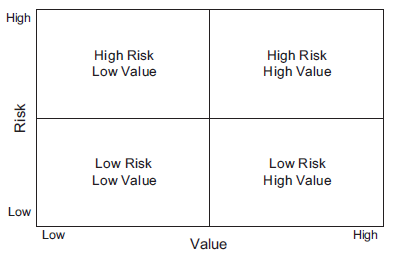
\includegraphics[scale=0.8]{relacao-risco-valor}
\end{figure}

A sequência apropriada é mostrada na Figura \ref{combinando-risco-e-valor}:

\begin{figure}
	\caption{Combinando risco e valor na priorização de funcionalidades}
	\label{combinando-risco-e-valor}
	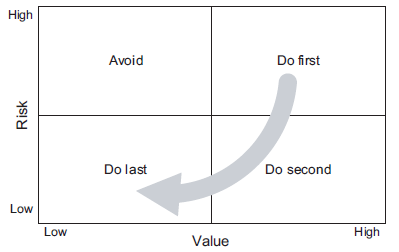
\includegraphics[scale=0.8]{combinando-risco-e-valor}
\end{figure}


É necessário ter em mente a classificação das funcionalidade pode e deve mudar com o progresso do projeto, sendo baseado nas histórias ainda não implementadas do product backlog.


\section{Combinando os quatro fatores}

A abordagem recomendada é fazer uma priorização inicial baseada em valor e custo. Após isto, conhecimento e risco podem ser usados para mover itens na lista de prioridades em um ajuste fino.

Não é necessário que esta seja uma atividade formal; ela pode estar simplesmente na cabeça do product owner e apresentada à equipe, que pode, com sua avaliação a respeito das funcionalidades, fornecer subsídios para manter ou alterar a priorização.


\section{Alguns exemplos}

Serão apresentados exemplos de priorização de temas em duas áreas: infraestrutura e projeto de interface com o usuário.

\subsection{Infraestrutura}

Considere um framework de segurança. Levando-se em conta que segurança é um item crítico e de alto valor para o cliente, a implantação da segurança deveria ser priorizada logo no início do projeto. Contudo, nenhuma aplicação é vendida apenas por ser segura; ela precisa antes servir para algo.

Com relação ao custo, como a segurança é um componente infraestrutural, provavelmente será mais barato incluí-la agora do que daqui a seis meses. Porém, quanto mais cedo se adiciona algo ao sistema, maior a probabilidade de que tenha que ser alterada conforme o conhecimento sobre o produto e sobre o projeto aumentam. Assim, o custo destas possíveis alterações também têm que ser pensados. Prevenir-se contra este custo é a idéia de ``decide as late as possible'' do Lean Software Development (Poppendieck).


\chapter{Priorização Financeira}

em breve...


\chapter{Priorizando desejabilidade}

em breve...


\chapter{Dividindo user stories}


\section{Quando dividir uma user story}
A divisão de user stories em unidades menores é útil quando:
\begin{itemize}
\item a estimativa de uma história é maior do que o esforço disponível para uma iteração única, seja porque a historia é realmente muito grande, seja porque o esforço que resta para a iteração é menor do que o esforço estimado para a história;
\item um épico necessita ser dividido de modo a possibilitar estimativas mais precisas.

\end{itemize}


\section{Dividindo por fronteiras de dados}

Uma estratégia de divisão de user stories é através das fronteiras dos dados suportados pela story. Por exemplo, uma story de um cadastro detalhado de dados de um cliente poderia ser dividida entre dados pessoais, contato e dados financeiros. Em um exemplo dado pelo livro, que não envolve CRUD diretamente, uma story para suporte a um subsistema de fax automatizado foi dividida entre suporte a números de telefone dos EUA e suporte a números internacionais.

\textit{\textbf{Divida uma user story grande com base nas fronteiras dos dados suportados por ela}}


\section{Dividindo por fronteiras operacionais}

Stories grandes podem ser divididas com base nas operações que são realizadas pela story. Tome um exemplo dado no livro: uma funcionalidade de busca com uma grande quantidade de campos e um grid complexo para mostrar os resutlados da consulta. Esta história foi dividida em funcionalidades, de modo que na primeira iteração, a busca apenas anunciava a quantidade de resultados obtidos. Mesmo isto não tendo valor para o cliente, constitui progresso visível. Na segunda iteração os dados foram apresentados de modo organizado e flexível.

\textit{\textbf{Divida uma user story grande com base nas operações realizadas por ela}}

Outra abordagem comum é dividir stories CRUD em suas partes constituintes.

\textit{\textbf{Divida uma user story grande em operações CRUD separadas}}


\section{Removendo funcionalidades ortogonais}

Uma história pode ser reduzida isolando-a de funcionalidades ortogonais como logging, manipulação de erros ou segurança. Por exemplo, GUIs que se comportam diferentemente dependendo do papel do usuário corrente, podem ter os comportamentos específicos implementados em iterações subsequentes. Ou, outro exemplo, uma consulta cujos resultados são vistos parcialmente dependendo do usuário pode primeiro ser implementada mostrando todos e só depois implementado o suporte a autorização. Validações são outro exemplo trazido pelo livro.

\textit{\textbf{Considere remover funcionalidades ortogonais (como logging, segurança, manipulação de erros etc.) e criar duas versões da user story: uma sem e outra com o suporte a estas funcionalidades}}


\section{Não satisfaça restrições de desempenho}

Imagine uma consulta que resulta na apresentação de uma série histórica. Devido à quantidade de dados envolvidos em consultas deste tipo, o desempenho pode ser uma requisito, exigindo técnicas como caching, database tuning e outras. Uma estratégia é separar a otimização da funcionalidade em si, o que pode ser generalizado para qualquer requisito não-funcional.

\textit{\textbf{Considere dividir uma user story grande através da separação entre aspectos funcionais e não-funcionais em user stories distintas}}


\section{Divida user stories com prioridade mista}

Uma abordagem para a divisão de uma user story grande é procurar por grãos de baixa prioridade e postergá-los a iterações posteriores. Por exemplo, uma funcionalidade de login pode ser dividida em
\begin{itemize}
\item usuário entra com nome e senha corretos, o sistema libera a entrada;
\item se o usuário entra com senha ou usuário inválido por mais de 3 vezes seguidas, o acesso é negado até um contato com o suporte;
\item quando o usuário tem o acesso negado, ele recebe um e-mail informando a situação.
\end{itemize}
Neste caso, a funcionalidade de login propriamente dito tem a prioridade mais alta e deve ser implementada primeiro.

\textit{\textbf{Separe uma user story grande em unidades menores se as prioridades destas unidades são diferentes}}



\section{Não separe uma história em tarefas}

Quando uma história é difícil de ser dividida, um modo fácil mas ruim de fazer isto é o seguinte:
\begin{itemize}
\item criar a interface do usuários
\item criar classes de negócio
\item criar tabelas
\end{itemize}

Isto não é aconselhável porque estas tarefas, tratadas independentemente, não trazem valor ao cliente. O correto é dividir em user stories que, mesmo que realizem pouco, sejam feitas inteiramente e atravessem todo o software e realizem uma ação completa.

\textit{\textbf{Não divida uma user story grande em tarefas. Em lugar disto, tente definir uma story que atravesse todas as camadas e apresente um resultado visível ao cliente}}


\section{Evite a tentação das mudanças relacionadas}

Uma vez que uma user story possui um tamanho adequado, resista à tentação de agregar funcionalidades aparentemente relacionadas, como, por exemplo, a correção de um pequeno bug no mesmo trecho de código onde a funcionalidade será implementada. Em casos como este, a priorização sempre deve ser levada em consideração.


\textit{\textbf{Não agregue atividades relacionadas a uma user story que já possui um tamanho adequado, a menos que as mudanças relacionadas tenham prioridade equivalente}}


\section{Combinando user stories}

Não existe regra que diga que o tamanho de uma user story (ou seja, a unidade de planejamento) tenha que ser a menor possível. Para iterações de 2 semanas, tamanhos que equivalem a durações de 2 a 5 dias são apropriados. Assim, pode ser útil também combinar histórias muito pequenas (que sejam relacionadas) em unidades maiores. Caso isto ocorra, a história resultante deve ser estimada como um todo. Um exemplo disto são correções de bugs minúsculos, que podem ser agregadas em uma história única de granularidade um pouco maior.




\chapter{Planejamento de release}


Planejamento de release é o processo de criação de um plano de alto nível que cubra um período maior que uma iteração. Um release típico tem duração de 3 a 6 meses. O planejamento de release é importante por várias razões:
\begin{itemize}
\item ajuda o product owner e a equipe a definir o quanto de funcionalidade será criada para o próximo release do produto;
\item define e dissemina as expectativas a respeito do que será desenvolvido e quando;
\item fornece uma linha de ação bem definida para a equipe. Sem o conceito de release, a equipe se move de uma iteração a outra em uma estrada sem fim.
\end{itemize}
Apenas com a visão da iteração, não há como enxergar claramente os objetivos maiores do projeto.

\section{O plano de release}

Parte do plano de release é definir o que pode ser feito e para quando. Alguns projetos definem uma data e as user stories são negociadas; outros definem uma lista de user stories absolutamente necessárias mas com prazo flexível. Além disto, o plano de release levar em consideração o valor do release para a organização.

Para determinar o quanto de funcionalidades podem ser incluídas em uma iteração, basta calcular levando em conta a quantidade de iterações desejada e a velocidade esperada ou conhecida da equipe. Por exemplo: um release para ser liberado em 6 meses com iterações de 2 semanas terá 13 iterações. Sabendo que a velocidade da equipe é de 20 pontos por iteração, a quantidade de esforço será de 20 x 13 = 260 story points. O plano de release é normalmente documentado simplesmente como uma lista de histórias selecionadas para o release.

No plano de release não constam informações a respeito de que desenvolvedores implementarão que user stories ou a priorização das user stories dentro do release. Estas questões são tratadas no planejamento da iteração (próximo capítulo).

Outras informações, como quem é a equipe, a duração das iterações, a quantidade delas, a data de início da primeira iteração e a data de término da última, podem ser adicionadas. E, naturalmente, outras que agregarem valor ao release em particular.

A Figura \ref{passos-para-o-planejamento-de-releases} mostra os passos para o planejamento dos releases.

\begin{figure}
	\caption{Passos para o planejamento de releases}
	\label{passos-para-o-planejamento-de-releases}
	\begin{center}
	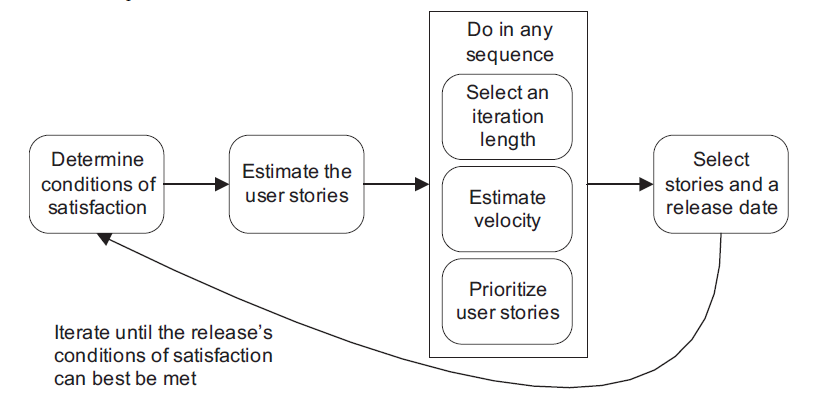
\includegraphics[scale=0.6]{passos-para-o-planejamento-de-releases}
	\end{center}
\end{figure}


\subsection{Determinando as condições de satisfação}

O product owner deve trazer os objetivos da organização com respeito ao release e definir uma lista de user stories que irá levar a estes objetivos.


\subsection{Estimar as user stories}

Todas as histórias do presente release devem ser estimadas. Ou seja, a equipe deve estimar todas as histórias que possuam uma razoável chance de figurarem no planejamento do release, de modo a fornecer subsídios para a priorização feita pelo product owner.


\subsection{Selecionar um tamanho de iteração}

Ver Capítulo \ref{selecionando-um-tamanho-de-iteracao}.


\subsection{Estimar velocidade}

A velocidade deve ser a média da velocidade que a equipe apresentou em outros projetos ou no release anterior. Caso a tecnologia, o domínio ou a equipe mudem bruscamente - ou simplesmente não haja este tipo de informação - podem ser usadas técnicas para estimar a velocidade (Capítulo \ref{capitulo-estimando-velocidade}) até que existam informações reais nas quais se basear.


\subsection{Priorizar user stories}

A priorização é responsabilidade do product owner, mas a equipe deve ser ouvida em relação e dependências e demais questões tecnológicas.


\subsection{Selecionando stories e uma data}

Se o projeto é feature-driven,
\begin{equation}
nº\;de\;iteracoes = \frac{\sum estimativas\;das\;stories}{velocidade\;esperada}
\end{equation}

Se o projeto é date-driven, o número de iterações pode ser obtido consultando-se o calendário. O número de story points disponível para o release é:
\begin{equation}
story\;points = nº\;de\;iteracoes * velocidade\;esperada
\end{equation}

Em relação ao detalhamento do plano de release, algumas equipes vinculam cada story a uma iteração, enquanto outras apenas definem as histórias sem vínculos prévios com iterações e deixam a decisão de que histórias serão incluídas em cada iteração para o planejamento da iteração.

Uma boa técnica para facilitar a discussão da inclusão ou não das histórias em um release é colocar todas em cartões e dividi-las em uma mesa, conforme a Figura \ref{iteracoes-em-colunas}.

\begin{figure}
	\caption{Distribuindo iterações em colunas}
	\label{iteracoes-em-colunas}
	\begin{center}
	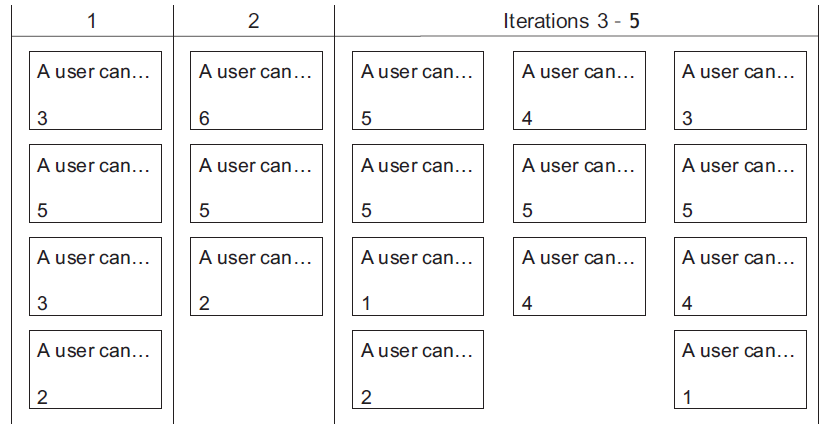
\includegraphics[scale=0.6]{iteracoes-em-colunas}
	\end{center}
\end{figure}


\section{Atualizando o plano de release}

O plano de release deve ser revisado frequentemente, e atualizado a critério dos envolvidos no projeto. Algumas equipes fazem isto à ocasião de cada planejamento de iteração.


\section{Um exemplo}

O exemplo é um website de torneios de natação. As user stories são as seguintes:
\begin{itemize}
\item Como um técnico, eu quero definir sessões de treinamento
\item Como um técnico, eu quero definir campos customizados que eu possa preencher para cada nadador
\item Como um nadador, eu quero tirar um relatório que mostre meus resultados em todos os eventos desde uma data fornecida
\item Como um nadador, eu quero atualizar minhas informações
\item Como um técnico, eu quero poder enviar um e-mail a todos os membros da equipe
\item Como um administrador do sistema, eu quero configurar permissões e grupos
\item Como um técnico, eu quero adquirir o software e usá-lo para a minha equipe
\item Como um nadador, eu quero comparar meus tempos com os recordes nacionais
\item Como um técnico, eu quero entrar os nomes e as informações de todos os nadadores da equipe
\item Como um nadador, eu quero ver meus melhores tempos em cada evento
\item Como um usuário, eu sou obrigado a me logar no sistema e eu posso ver apenas os dados para os quais tenho permissão
\item Como um nadador, eu quero ver todos os meus tempos para um evento específico
\end{itemize}

\subsection{Determinando as condições de satisfação}

O início da temporada é daqui a quatro meses. O software deve estar disponível um mês antes. O product owner deve incluir tantas funcionalidades quanto possível, mas a principal restrição é o tempo. Algo deve ser lançado em três meses, nem que seja apenas o básico para pequenas equipes. O custo é fixo e o pessoal disponível constitui-se de um programador, um administrador de banco de dados e um testador, que já fazem parte da equipe.

\subsection{Estimando}

Os três desenvolvedores estimam as histórias em uma reunião com o product owner, que fornece os esclarecimentos necessários. A equipe faz a estimativa que consta da Tabela \ref{tabela-com-as-estimativas}.

\begin{table}
  \caption{Lista priorizada de histórias}
  \label{tabela-com-as-estimativas}
  \begin{center}
    \begin{tabular}{clr}
      \hline
      &\textbf{User Story}&\textbf{Estimativa}\\
      \hline
      &Como um técnico, eu quero adquirir o software e usá-lo para a minha equipe&5\\
      &Como um usuário, eu sou obrigado a me logar no sistema e eu posso ver apenas os dados para os quais tenho permissão&5\\
      &Como um técnico, eu quero entrar os nomes e as informações de todos os nadadores da equipe&8\\
      &Como um nadador, eu quero ver todos os meus tempos para um evento específico&5\\
      &Como um nadador, eu quero atualizar minhas informações&5\\
      &Como um nadador, eu quero ver meus melhores tempos em cada evento&5\\
      &Como um nadador, eu quero tirar um relatório que mostre meus resultados em todos os eventos desde uma data fornecida&5\\
      &Como um nadador, eu quero comparar meus tempos com os recordes nacionais&8\\
      &Como um técnico, eu quero definir sessões de treinamento&8\\
      &Como um técnico, eu quero poder enviar um e-mail a todos os membros da equipe&3\\
      &Como um técnico, eu quero definir campos customizados que eu possa preencher para cada nadador&8\\
      &Como um administrador do sistema, eu quero configurar permissões e grupos&3\\
      \hline
      &\textbf{Total}&\textbf{68}\\
      \hline
    \end{tabular}
  \end{center}
\end{table}

\subsection{Estimando o tamanho da iteração}

Como o projeto irá durar apenas 3 meses, os desenvolvedores e product owner concordam que 4 semanas é muito tempo para a duração da iteração. Baseado nos pontos que serão apresentados no Capítulo \ref{selecionando-um-tamanho-de-iteracao}, a decisão é por iterações de 2 semanas.


\subsection{Estimando a velocidade}

O projeto contará com dois desenvolvedores e um testador. Usando técnicas que constam no Capítulo \ref{capitulo-estimando-velocidade}, é estimada uma velocidade de 8 pontos por iteração.


\subsection{Priorizando as user stories}

O product owner, baseado em pesquisas e entendimento prévio, prioriza as histórias de acordo com o mostrado na Tabela \ref{tabela-com-as-estimativas}.


\subsection{Selecionando as user stories}

Sabendo que em três meses é possível ter 6 iterações de 2 semanas (com 1 semana de sobra para acomodar eventualidades) e que a velocidade estimada da equipe é de 8 pontos por iteração, temos um total de 48 disponíveis para serem implementados para o release.

O caminho então é fazer um corte na lista de histórias, selecionando as mais prioritárias até 48 pontos, o que iria até a história ``Como um nadador, eu quero comparar meus tempos com os recordes nacionais'', somando um total de 46 pontos, valor suficientemente próximo a 48 para que o product owner concorde que a lista para o release termine aí.

Porém, a última história, ``Como um administrador do sistema, eu quero configurar permissões e grupos'', apesar da baixa prioridade, é absolutamente necessária. A história foi estimada para 3 pontos, e, caso entre no release, o elevaria a 49 pontos. A maioria das equipes, nestas circunstâncias, concordaria com a inclusão. A equipe do exemplo, porém, não concordou.

Assim, o product owner decidiu remover a história ``Como um nadador, eu quero comparar meus tempos com os recordes nacionais'', deixando a lista escolhida com 41 pontos. Aqui ele poderia adicionar a história ``Como um técnico, eu quero poder enviar um e-mail a todos os membros da equipe'', que possui 3 pontos. Porém, preferiu deixar com 41 para decidir depois, caso o projeto fique adiantado, incluir a história de 8 pontos que foi removida. Isto faz o plano do release ficar conforme a Tabela \ref{plano-de-release-final}.

\begin{table}
  \caption{Plano de release final}
  \label{plano-de-release-final}
  \begin{center}
    \begin{tabular}{clr}
      \hline
      &\textbf{User Story}&\textbf{Estimativa}\\
      \hline
      &Como um técnico, eu quero adquirir o software e usá-lo para a minha equipe&5\\
      &Como um administrador do sistema, eu quero configurar permissões e grupos&3\\
      &Como um usuário, eu sou obrigado a me logar no sistema e eu posso ver apenas os dados para os quais tenho permissão&5\\
      &Como um técnico, eu quero entrar os nomes e as informações de todos os nadadores da equipe&8\\
      &Como um nadador, eu quero ver todos os meus tempos para um evento específico&5\\
      &Como um nadador, eu quero atualizar minhas informações&5\\
      &Como um nadador, eu quero ver meus melhores tempos em cada evento&5\\
      &Como um nadador, eu quero tirar um relatório que mostre meus resultados em todos os eventos desde uma data fornecida&5\\
      \hline
      &\textbf{Total}&\textbf{41}\\
      \hline
    \end{tabular}
  \end{center}
\end{table}


\chapter{Planejamento da iteração}

O planejamento da iteração fornece uma visão mais detalhada sobre o projeto, sendo realizado em uma reunião na qual participam a equipe, o product owner e qualquer outra pessoa que for necessária (especialistas do negócio, marketing etc). 

O plano da iteração pode tomar a forma de uma planilha (Figura \ref{plano-da-iteracao-como-tabela}) ou um conjunto de cartões escritos à mão (Figura \ref{plano-da-iteracao-como-cartoes}) e distribuídos sobre uma mesa. Independente da forma, deve ser simples ligar tarefas às suas respectivas user stories. Para equipes não distribuídas, a abordagem de cartões é a mais indicada. O uso de planilhas diminui a capacidade de discussão e dá um poder muito maior a quem está manipulando o computador durante a discussão. Com o uso de cartões, qualquer um pode escrever tarefas e a visualização e a manipulação das tarefas fica facilitada.

\begin{figure}
  \caption{Plano da iteração mostrado como uma tabela}
  \label{plano-da-iteracao-como-tabela}
  \begin{center}
  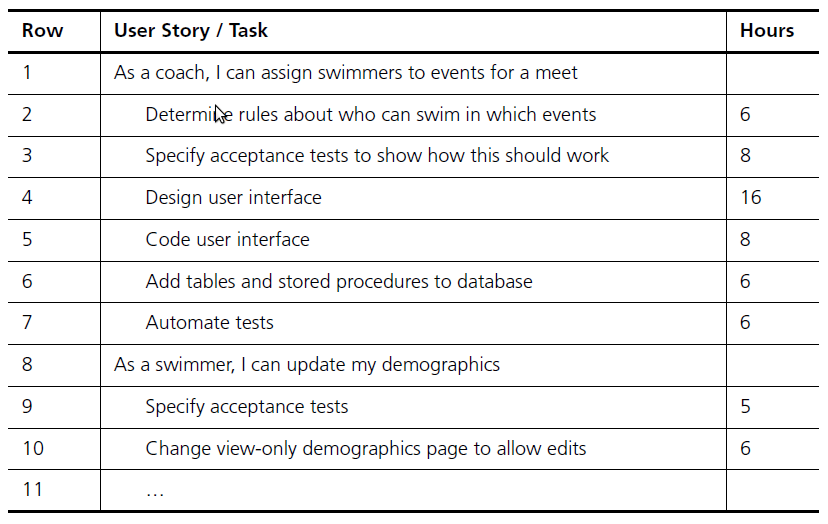
\includegraphics[scale=0.6]{plano-da-iteracao-como-tabela}
  \end{center}
\end{figure}

\begin{figure}
  \caption{Plano da iteração com cartões em uma mesa}
  \label{plano-da-iteracao-como-cartoes}
  \begin{center}
  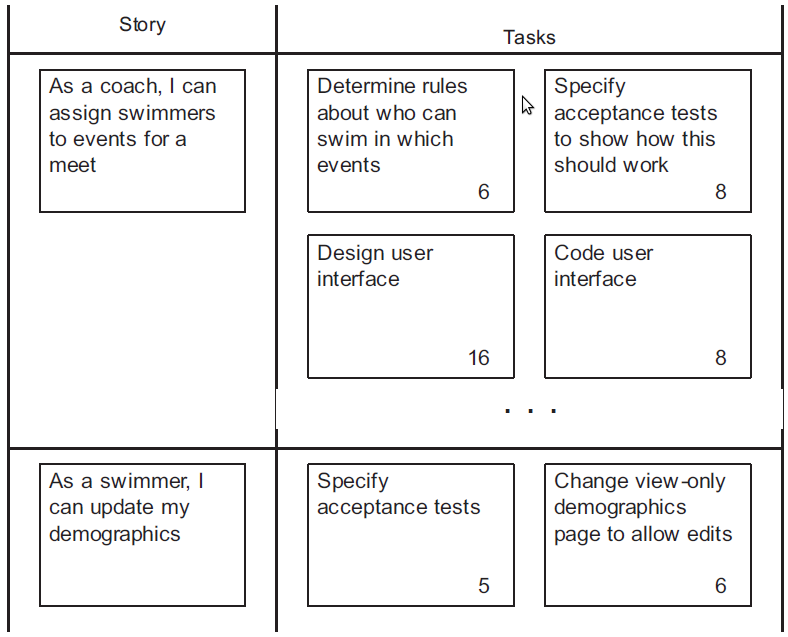
\includegraphics[scale=0.6]{plano-da-iteracao-como-cartoes}
  \end{center}
\end{figure}


\section{Não há alocação de tarefas durante o planejamento da iteração}

Durante o planejamento da iteração não deve haver nenhuma alocação de tarefas a desenvolvedores, por mais que para algumas tarefas pareça óbvio quem fará o quê. Cada desenvolvedor só estará alocado a uma tarefa de cada vez (talvez duas, caso relacionadas) e só pegará uma segunda tarefa ao término da primeira. Além disto, dividir previamente a iteração entre os desenvolvedores pode minar o senso de equipe e a colaboração necessárias a um projeto ágil.

\section{Como o planejamento da iteração difere do planejamento do release}

No planejamento da iteração, as user stories levantadas no planejamento do release são decompostas em tarefas. Enquanto histórias são estimadas em story points ou dias ideais, tarefas são estimadas em horas ideais. As principais diferenças entre os planejamentos de iteração e de release são mostrados na Tabela \ref{diferencas-entre-planejamento-iteracao-e-release}.

\begin{table}
  \caption{Principais diferenças entre planejamento de iteração e de release}
  \label{diferencas-entre-planejamento-iteracao-e-release}
  \begin{center}
    \begin{tabular}{c c c}
      \hline
       &\textbf{Planejamento de release}&\textbf{Planejamento de iteração}\\
      \hline
      Horizonte de planejamento&3 a 9 meses&1 a 4 semanas\\
      Itens no plano&User stories&Tarefas\\
      Estimado em&Story points ou dias ideais&Horas ideais\\
      \hline
    \end{tabular}
  \end{center}
\end{table}

O planejamento ágil funciona em dois estágios: o primeiro, planejamento de release, tem uma visão de alto nível e é intencionalmente vago; o segundo, o planejamento de iteração, é muito mais detalhada e seu nível de imprecisão é bem menor. 

O planejamento da iteração envolve discussões a respeito de design de produto (melhor combinação de histórias para maximizar o ROI, interpretações do feedback dos clientes, decisões a respeito se uma funcionalidade merece (worth) ser implementada ou não etc.) e design de software (questões arquiteturais e tecnológicas, reúso de código etc.).  Como o planejamento da iteração está temporalmente muito próximo da implementação real, o nível de especulação destas discussões é baixíssimo, pois se trata de coisas que serão realizadas quase instantaneamente.

\section{Planejamento de iteração guiado por velocidade}

Os passos envolvidos no planejamento de iteração guiado por velocidade são mostrados na Figura \ref{planejamento-de-iteracao-guiado-por-velocidade}.

\begin{figure}
  \caption{Sequência de passos no planejamento de iteração guiado por velocidade}
  \label{planejamento-de-iteracao-guiado-por-velocidade}
  \begin{center}
  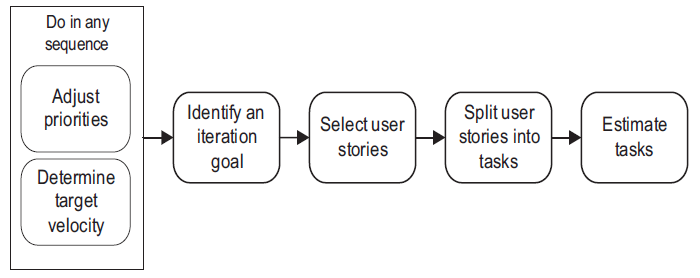
\includegraphics[scale=0.6]{planejamento-de-iteracao-guiado-por-velocidade}
  \end{center}
\end{figure}


\subsection{Ajustar prioridades}

Embora a lista de histórias seja ordenada por prioridades no planejamento do release, as condições podem mudar com o tempo e o planejamento da iteração deve contemplar a possibilidade de ajuste das prioridades.

A reunião de revisão da iteração que ocorre ao final da iteração, por exemplo, é uma ocasião onde podem ocorrer ajustes nas prioridades. Nesta reunião, a equipe demonstra ao product owner, stakeholders e demais interessados, com software funcionando, o progresso obtido na iteração. O feedback gerado nestas reuniões pode levar a alterações na priorização.


\subsection{Determinar a velocidade}

A velocidade da equipe para a iteração que se inicia tende a ser semelhante à velocidade na iteração que terminou (ver \textit{yesterday weather} em Planning Extreme Programming, de Kent Beck e Martin Fowler, 2000). Outras equipes fazem uma média das últimas iterações. Caso a equipe não tenha dados anteriores de velocidade, ver Capítulo \ref{capitulo-estimando-velocidade}.


\subsection{Identificar o objetivo da iteração}

O objetivo da iteração é uma meta que deve nortear os esforços de todos durante a iteração. Exemplos:
\begin{itemize}
 \item Realizar progressos na construção dos relatórios
 \item Implementar segurança
\end{itemize}

O objetivo da iteração não deve ser específico demais, ou seja, devem ser evitadas coisas como ``Finalizar 15 relatórios''.


\subsection{Selecionar user stories}

As histórias selecionadas devem combinar com o objetivo da iteração. Se o objetivo é: ``Todos os cadastros de dados sobre os nadadores devem ser finalizados'', as histórias escolhidas seriam:
\begin{itemize}
 \item Como um nadador, eu quero atualizar meus dados
 \item Como um técnico, eu quero inserir dados para todos os nadadores
 \item Como um técnico, eu quero importar um arquivo com todos os dados
 \item Como um técnico, eu quero exportar um arquivo com todos os dados
\end{itemize}
A seleção das histórias deve respeitar a priorização. Se a quarta história, por exemplo, tiver uma prioridade muito baixa, ela pode ser removida, a critério do product owner. Assim, o objetivo passará a ser ``Os cadastros de dados mais importantes sobre os nadadores devem ser finalizados''.


\subsection{Dividir user stories em tarefas}

No planejamento da iteração, cada história deve ser dividida nas tarefas necessárias à sua implementação. A Figura \ref{plano-da-iteracao-como-tabela} mostra um exemplo. Todas as tarefas importantes, de levantamento de requisitos a documentação de usuário, devem ser incluídas.

\subsubsection{Apenas inclua trabalho que adicione valor diretamente ao projeto}

Somente devem ser criadas tarefas \textbf{diretamente} relacionadas ao projeto. Coisas como Responder e-mails, preencher softwares de acompanhamento de tarefas (mesmo que sejam e-mails e tarefas relacionados ao projeto) ou reuniões sobre processo não fazem parte da construção do produto e não devem ser incluídas.

\subsubsection{Reuniões contam (pra c***)}

Se houver tarefas que sejam reuniões, o tempo de todos os participantes deve ser incluído. Se sete membros da equipe irão participar de uma reunião de uma hora e o líder técnico planeja gastar 2 horas preparando a reunião, o tempo estimado deve ser de 9 horas (7 * 1 + 2).

\subsubsection{Bugs}

Uma equipe ágil tem como meta resolver bugs na iteração na qual são encontrados. Caso isto não ocorra, os bugs devem ser encarados como uma história normal, ou, caso sejam muito pequenos, resolvidos em conjunto como uma história única, que só termina quando todos os testes passam.

\subsubsection{Lidando com dependências}

Não há problema quando as dependências seguem a ``ordem natural''. Ordem natural aqui é entendida como a ordem que a equipe levou em consideração ao estimar as user stories. Por exemplo: imagine uma história de inclusão de dados e outra de visualização de dados. A ``ordem natural'' é incluir primeiro e visualizar depois. Na estimativa da inclusão é levado em conta o esforço de criação de tabelas; na exclusão não. Se a ``ordem natural'' é invertida, a implementação da exclusão demandará a criação do banco e a inclusão diretamente no banco de alguns dados.

Porém, isto provavelmente não significa que o esforço geral aumentará, apenas algumas tarefas migrarão de uma história para outra (noexemplo, ``criar tabelas'' sairá da história de inclusão e irá para exclusão). De acordo com o autor, atender às expectativas do product owner é mais importante e isto não é um motivo para maiores preocupações. Além disto, mesmo que isto acarretasse em algum atraso, o product owner (que zela pelo ROI do projeto) decerto tem boas razões de negócio para este tipo de exigência.


\subsubsection{Trabalho que é difícil de dividir}

Geralmente, dificuldades em dividir histórias se devem ao desconhecimento de detalhes a respeito da implementação. Em casos assim, pode-se fazer uso de tarefas denominadas \textit{spikes}, que são tarefas exploratórias para se descobrir ou aprender sobre algo. Assim, uma história com esse tipo de problema poderia ser dividida assim:
\begin{itemize}
 \item Determinar a extensão do problema, 2 horas
 \item Realizar as tarefas necessárias, 10 horas
\end{itemize}

A primeira tarefa é o spike, a segunda é pouco mais que um chute e poderá ser, após o spike, refinada.


\subsection{Estimar tarefas}

O próximo passo é estimar cada tarefa, sempre usando unidades ideais de tempo (ou seja, uma tarefa de 4 horas ideais pode eventualmente ocupar um dia inteiro, caso haja muitas interrupções, reuniões etc). É importante que as estimativas devem sempre ser feitas em conjunto por toda a equipe.

\subsubsection{Não há problema em (um pouco de) design}

Alguma discussão a respeito de design eventualmente será necessária para as estimativas. Um bom sinal para perceber quando se deve parar de discutir design no planejamento da iteração é quando alguém pensa em desenhar um diagrama. É um sinal de que se está indo longe demais. Caso se descubra ao implementar que houve enganos na estimativa ou mesmo na formulação de algumas tarefas, elas devem ser revisadas junto ao product owner.

\subsubsection{O tamanho certo para a tarefa}

O tamanho ideal de cada tarefa é aquele no qual um desenvolvedor seja capaz de realizar em no máximo dia, de modo que ao fim de cada dia haja pelo menos uma tarefa completa para ser reportada. Tarefas maiores devem ser entendidas como temporárias, até que maior informação seja obtida de modo a se poder quebrá-las.


\section{Planejamento da iteração guiado por comprometimento}

Os passos envolvidos no planejamento de iteração guiado por comprometimento são mostrados na Figura \ref{planejamento-de-iteracao-guiado-por-comprometimento}.

\begin{figure}
  \caption{Sequência de passos no planejamento de iteração guiado por comprometimento}
  \label{planejamento-de-iteracao-guiado-por-comprometimento}
  \begin{center}
  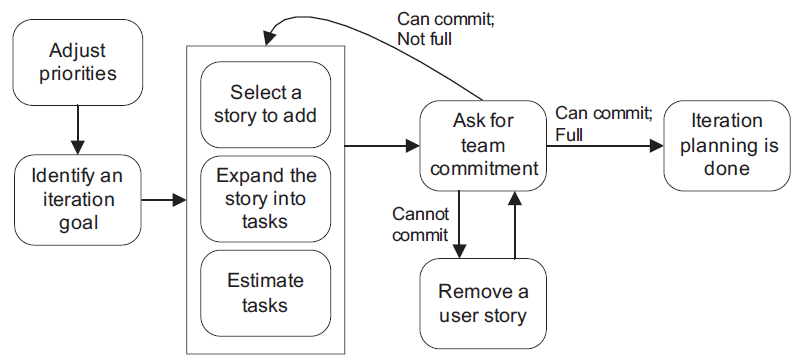
\includegraphics[scale=0.6]{planejamento-de-iteracao-guiado-por-comprometimento}
  \end{center}
\end{figure}

Os primeiros passos - ajustar prioridades e identificar o objetivo da iteração - são iguais à abordagem guiada por velocidade. O grupo seguinte (3 passos) também é semelhante, com a diferença de que é feito apenas para uma história de cada vez.

\subsection{Verificar o comprometimento da equipe}

É importante que o comprometimento da equipe seja com a entrega de funcionalidades e não simplesmente com completar um conjunto de tarefas. Isto faz diferença, por exemplo, quando surge uma nova tarefa no meio de uma iteração, fato que deve ser ou implementada simplesmente (caso não impacte no planejamento da iteração) ou discutida com o product owner para revisões no planejamento.

Na abordagem guiada por comprometimento, não é usado o conceito de velocidade para determinar quando histórias suficientes foram incluídas na iteração, mas sim o quanto a equipe se compromete como sendo capaz de implementar na iteração.

\subsubsection{Somando as estimativas}

Um bom modo de verificar se o comprometimento da equipe é realista, é somar as estimativas em horas ideais das histórias e comparar com as horas reais disponíveis. Por exemplo, se há 560 horas reais disponíveis, estimativas realistas devem oscilar entre 280 e 420 horas ideais.

Deve ser verificada também os tipos de tarefas e as diferentes habilidades na equipe, de modo que não haja um excesso de tarefas que só possam ser realizadas por poucos desenvolvedores.

\subsubsection{Manutenção e comprometimento}

É comum que equipes que estão implementando um software também estejam comprometidas com a manutenção de softwares preexistentes. Se este for o caso, o esforço de manutenção deve ser levado em conta no comprometimento com o software sendo criado. A Figura \ref{copo-do-comprometimento} usa a analogia com um copo com líquido para demonstrar este conceito.

\begin{figure}
  \caption{O copo do comprometimento}
  \label{copo-do-comprometimento}
  \begin{center}
  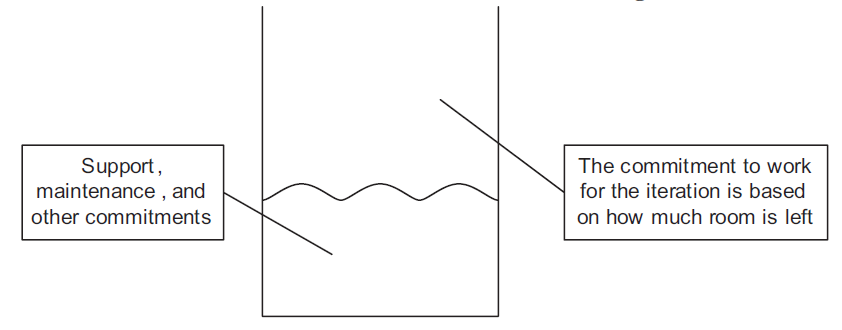
\includegraphics[scale=0.6]{copo-do-comprometimento}
  \end{center}
\end{figure}

Quando a equipe não sabe de antemão exatamente quais serão suas demandas extras, uma média pode ser aplicada. A situação ideal é evitar tanto quanto possível sobrecarregar a equipe com duas responsabilidades.


\section{Minha recomendação}

A preferência do autor é pela planejamento de iteração baseado em comprometimento, por considerar que o conceito de velocidade é adequado para planejamento de releases, mas não é preciso o suficiente para estimativas de granularidade fina como iterações.


\section{Relacionando estimativas de tarefas a story points}

Através do conceito de velocidade, é possível relacionar o número de horas ideais de uma iteração com o número de story points estimados. Este número, porém, não pode ser tomado como absoluto. Imaginando-se, que para uma determinada equipe, 1 story point foi calculado como equivalente a 12 horas, o comportamento real tende a ser como nas Figuras \ref{distribuicao-de-tempo-para-historia-de-1-ponto} e \ref{distribuicao-de-tempo-para-historias-de-1-2-e-3-pontos}.

\begin{figure}
  \caption{Distribuição de tempo para histórias de 1 ponto}
  \label{distribuicao-de-tempo-para-historia-de-1-ponto}
  \begin{center}
  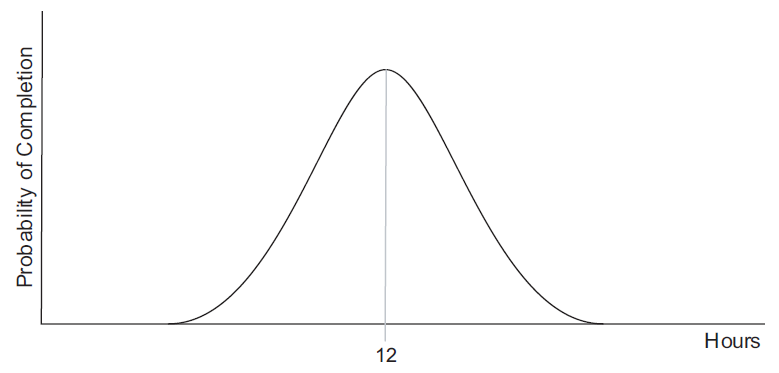
\includegraphics[scale=0.6]{distribuicao-de-tempo-para-historia-de-1-ponto}
  \end{center}
\end{figure}


\begin{figure}
  \caption{Distribuição de tempo para histórias de 1, 2 e 3 pontos}
  \label{distribuicao-de-tempo-para-historias-de-1-2-e-3-pontos}
  \begin{center}
  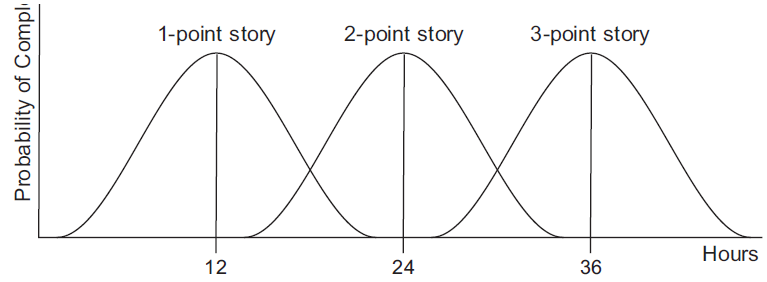
\includegraphics[scale=0.6]{distribuicao-de-tempo-para-historias-de-1-2-e-3-pontos}
  \end{center}
\end{figure}


\chapter{Selecionando um tamanho de iteração}
\label{selecionando-um-tamanho-de-iteracao}

Normalmente, iterações em projetos ágeis vão de 1 a 4 semanas. Porém, o tamanho correto varia de projeto para projeto.

\section{Fatores na seleção do tamanho da iteração}

A duração da iteração deve ser guiada pelos seguintes fatores:
\begin{itemize}
 \item o tamanho do release que conterá as iterações;
 \item a quantidade de incerteza;
 \item a facilidade de obter feedback;
 \item por quanto tempo as prioridades podem se manter inalteradas;
 \item o overhead associado a cada iteração;
 \item a uniformidade do sentimento de urgência.
\end{itemize}

\subsection{O tamanho do release}

O tamanho da iteração influi:
\begin{itemize}
 \item na frequência com que novas versões do software serão liberadas para clientes e usuários;
 \item na frequência com que o progresso do projeto será mensurado e percebido;
 \item na frequência com que planos e priorizações serão revisados.
\end{itemize}

A recomendação é que o tamanho da iteração deve ser tal que permita que em um release aconteçam no mínimo 5 ocasiões onde os pontos listados possam ocorrer.


\subsection{A quantidade de incerteza}

Quanto mais incerteza, tanto em aspectos de requisitos, quanto aspectos de processo ou técnicos, mais curtas devem ser as iterações.


\subsection{A facildade de obter feedback}

A duração da iteração deve levar em consideração as características da organização: se só for possível ter a atenção dos stakeholders em situações formais, as iterações devem ser mais curtas. O objetivo é maximizar o feedback.


\subsection{Por quanto tempo as prioridades podem se manter inalteradas}

\textbf{É importantíssimo que as prioridades não sejam alteradas durante uma iteração}. Assim, o tamanho da iteração deve ser tal que permita que novas prioridades esperem até seu final. O tempo médio para que uma nova idéia se torne software em funcionamento é de uma iteração e meia, conforme a Figura \ref{tempo-para-uma-nova-ideia-virar-software}. Se mudanças de prioridades são muito frequentes, iterações mais curtas são mais indicadas. 

\begin{figure}
  \caption{Distribuição de tempo para histórias de 1 ponto}
  \label{tempo-para-uma-nova-ideia-virar-software}
  \begin{center}
  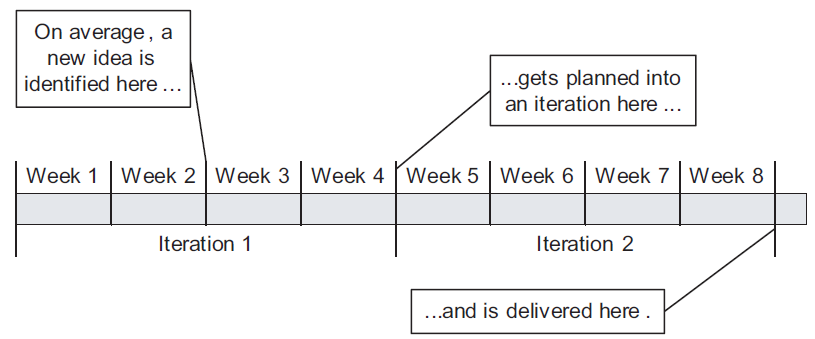
\includegraphics[scale=0.6]{tempo-para-uma-nova-ideia-virar-software}
  \end{center}
\end{figure}


\subsection{O overhead associado à iteração}

Toda iteração possui um overhead associado: reuniões, deployment, revisões, planejamento etc. Embora o objetivo de uma equipe ágil seja minimizar o overhead, este deve ser levado em conta ao escolher um tamanho de iteração.


\subsection{O sentimento de urgência é mantido}

Todo prazo pode levar a um relaxamento no início e uma pressão por resultados no final. Iterações menores diminuem isto ao distribuir mais uniformemente o stress, em lugar de concentrá-lo no final.


\section{Tomando uma decisão}

A preferência do autor é por iterações de duas semanas. Segundo ele, iterações mais longas (4 semanas, por exemplo), se por um lado permitem maior investigação e a elaboração de soluções mais criativas, por outro lado, têm o efeito de um grande relaxamento no início e um stress ao final. Iterações mais curtas (1 semana) tendem a ser muito estressantes e deixam pouco espaço para recuperar falhas\footnote{Nota de Rodrigo: Por outro lado, uma das práticas primárias do XP é justamente o ciclo semanal}.

\subsection{6x2+1}

Uma boa prática para eliminação de dívida técnica\footnote{http://martinfowler.com/bliki/TechnicalDebt.html, acesso em 31/03/2010} é ter seis iterações seguidas (no caso, de 2 semanas) e uma iteração de uma semana dedicada à melhoria de aspectos técnicos que os desenvolvedores julgarem relevante.



\chapter{Estimando velocidade}
\label{capitulo-estimando-velocidade}

Há 3 formas de estimar a velocidade de uma equipe:
\begin{itemize}
 \item usar valores históricas;
 \item realizar uma iteração;
 \item fazer uma previsão.
\end{itemize}

É importante ter em mente que a velocidade, por ser uma medida imprecisa, deve ser acompanhada de uma faixa. Por exemplo, se a velocidade estimada é de 20 pontos por iteração, é prudente estabelecer que a velocidade da equipe está entre 16 e 24 pontos por iteração.


\section{Usar valores históricos}

Para que valores históricos de velocidade sejam válidos, alguns fatores precisam ser os mesmos:
\begin{itemize}
 \item tecnologia;
 \item domínio;
 \item equipe;
 \item product owner;
 \item ferramentas;
 \item ambiente de trabalho;
 \item pessoas que fazem as estimativas.
\end{itemize}

A resposta normalmente é sim entre releases do mesmo projeto, mas não entre projetos diferentes. Uma boa forma de estimar a velocidade nestes casos é tirar a média das últimas iterações e aplicar uma faixa de incerteza.

\section{Realizar uma iteração}

A maneira ideal de estimar velocidade é realizar uma (idealmente duas ou três) iterações e estimar a velocidade a partir da velocidade observada. Esta deve ser a abordagem padrão, a ser utilizada sempre que possível. À medida que a quantidade de iterações aumenta, a incerteza diminui, conforme a Figura \ref{cone-da-incerteza} e a Tabela \ref{multiplicadores-de-incerteza}.


\begin{figure}
  \caption{O cone da incerteza}
  \label{cone-da-incerteza}
  \begin{center}
  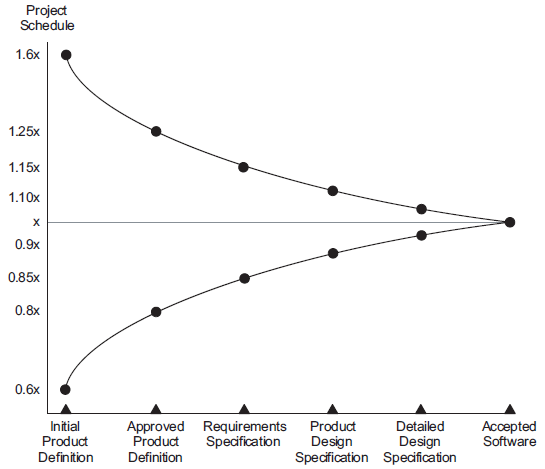
\includegraphics[scale=0.6]{cone-da-incerteza}
  \end{center}
\end{figure}

\begin{table}
  \caption{Multiplicadores de incerteza e quantidade de iterações}
  \label{multiplicadores-de-incerteza}
  \begin{center}
    \begin{tabular}{c c c}
      \hline
       \textbf{Iterações completas}&\textbf{Multiplicador menor}&\textbf{Multiplicador maior}\\
      \hline
      1&0.6&1.6\\
      2&0.8&1.25\\
      3&0.85&1.15\\
      4 ou mais&0.9&1.1\\
      \hline
    \end{tabular}
  \end{center}
\end{table}


\section{Fazer uma previsão}

Previsões de velocidade devem ser utilizadas em último caso, quando não existem dados históricos nem é possível realizar iterações para observar a velocidade. Estas estimativas possuem um alto grau de incerteza. Os passos para prever a velocidade são:

\begin{enumerate}
 \item Estimar o número de horas disponíveis de cada pessoa no projeto.
 \item Determinar o número total de horas que serão gastas durante a iteração.
 \item Selecionar histórias, estimá-las, dividi-las em tarefas, e também estimá-las até que o número de horas da iteração seja alcançado.
 \item Calcular a velocidade com base nas histórias selecionadas e aplicar uma faixa.
\end{enumerate}

\subsection{Estimando as horas disponíveis}

Em uma equipe, as pessoas não dedicam a totalidade de seu dia na implementação de funcionalidades. Estimativas a respeito da porcentagem de tempo gasto em trabalho efetivo (ou seja, aquele utilizado para trabalhar nas tarefas) variam entre 55\% e 80\%. Estas porcentagens devem ser levadas em consideração na estimativa de horas disponíveis.

\subsection{Estimar o tempo disponível em uma iteração}

Simples: 

número de horas disponíveis por dia x número de pessoas na equipe x número de dias em cada iteração.

Detalhes como feriados e férias não são significativos a ponto de terem que ser considerados, além do fato de que as disponibilidades dos membros da equipe não são estimadas a 100%.

\subsection{Expandir histórias até preencherem o tempo disponível}

Escolha um conjunto representativo de histórias, divida as histórias em tarefas e estime s tarefas. Isto deve ser feito até que a quantidade de horas estimadas iguale a quantidade disponível. 

\subsection{Aplique uma faixa}

A velocidade pode ser derivada da estimativa das histórias em pontos. À velocidade calculada deve ser aplicada uma porcentagem de -60\% a 160\%.

\subsection{Uma variação para algumas equipes}

Em equipes onde a quantidade de tempo disponível de cada membro da equipe é diferente, a disponibilidade deve ser o somatório das horas disponíveis de cada membro.


\section{Que abordagem eu deveria usar?}

Em ordem de preferência, as abordagens preferenciais devem ser:
\begin{enumerate}
 \item a realização de uma ou mais iterações. Nada substitui a observação de uma iteração real;
 \item usar a velocidade real de um projeto relacionado feito pela equipe;
 \item estimar a velocidade.
\end{enumerate}



\chapter{Amortecendo incertezas no plano}

Em algumas situações, projetos ágeis têm dificuldades em manter um escopo negociável, tendo restrições pesadas em termos de escopo e tempo. Nestes casos, as técnicas de planejamento vistas até aqui podem ser insuficientes, necessitando da adoção de um mecanismo que amorteça (\textit{buffering}) as incertezas.

\subsection{Buffers de funcionalidade}

O todo de user stories é dividido em imprescindíveis e desejáveis. Garante-se as imprescindíveis implementando-as primeiro, permitindo assim que as incertezas sejam absorvidas na implementação das histórias que são apenas desejáveis. [Nota de Rodrigo: Se o product backlog está corretamente priorizado, isto já acontecerá naturalmente]

\subsection{Buffers de tempo}

Consistem na inclusão de um ``sobretempo'' às estimativas de modo a absorver incertezas.

\subsubsection{Refletindo a incerteza nas estimativas}

Para protejer um projeto da incerteza, ela precisa ser quantificada. A Figura \ref{distribuicao-do-tempo-para-completar-uma-tarefa} mostra a distribuição dos tempos necessários para se completar uma tarefa. A cauda da direita é mais longa porque não é muito comum uma tarefa ser terminada muito antes do tempo médio mas há inúmeras situações que podem atrasar bastante a implementação de uma tarefa.

\begin{figure}
  \caption{Distribuição do tempo necessário para completar uma tarefa}
  \label{distribuicao-do-tempo-para-completar-uma-tarefa}
  \begin{center}
  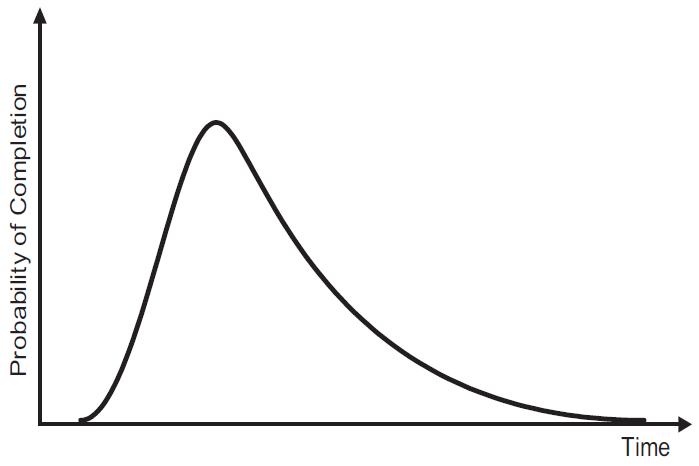
\includegraphics[scale=0.6]{distribuicao-do-tempo-para-completar-uma-tarefa}
  \end{center}
\end{figure}


more coming soon...


\chapter{Planejamento projetos multi-equipe}

coming soon...



\chapter{Monitorando o plano do release}

A execução do plano do release não é uma linha reta: podem ocorrer mudanças ou refinamento nos requisitos, a taxa de progresso pode não ser a esperada, podem ter ocorrido erros no planejamento. Assim, é preciso monitorar continuamente o plano para assegurar sua validade no tempo.

\section{Monitorando o release}

A importância do monitoramento do release pode ser demonstrada por um exemplo: imagine que o product owner decidiu incluir 40 story points ao release e a equipe já completou 30. Ela está, neste momento, mais longe do fim do release de que estava quando nada ainda havia sido feito. Neste caso, o fim do release terá que ser deslocado para frente ou algo terá que sair do release. Ou seja, o release deve ser replanejando. Do mesmo modo, a equipe pode aprender algo que a faz reestimar as histórias (ver Capítulo \ref{capitulo-reestimando}).

\subsection{Velocidade}

Dada a importância da velocidade como principal métrica de progresso de uma equipe ágil, é preciso seguir algumas regras para calculá-la. A mais importante é que para o cálculo da velocidade entram apenas as user stories \textbf{completas} ao fim da iteração. Por uma história ``completa'' entende-se escrita, refatorada, integrada e com todos os testes e inspeções passando. Créditos parciais não são aceitos por 3 motivos principais: são difíceis de mensurar, não reforçam a confiança do cliente no projeto pois ele não vê resultados concretos e aumenta o work-in-progress, que diminui a frequência de funcionalidades entregues. Para evitar histórias incompletas, o ideal é ter histórias tão pequenas quanto possível.

Mais importante do que a questão de como computar histórias incompletas é trabalhar para evitar que elas existam, através de esforços para elaborar histórias menores e melhores estimativas.


\section{Burndown charts do release}

O burndown chart é um mecanismo de demonstrar visualmente o andamento de um projeto, e se compõe de dois eixos, o horizontal com as iterações e o vertical com o esforço. A Figura \ref{burndown-completo} mostra um projeto de 240 pontos terminado em 8 iterações.

\begin{figure}
  \caption{Um projeto de 240 pontos completo em 8 iterações}
  \label{burndown-completo}
  \begin{center}
  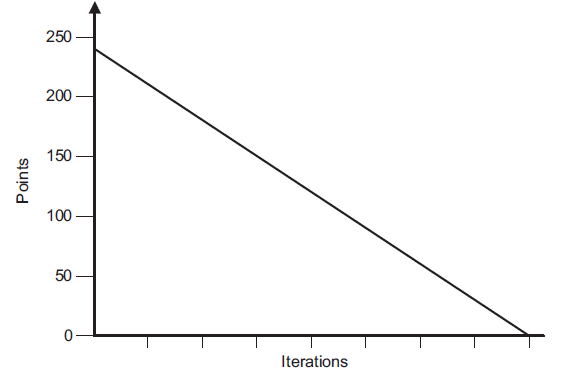
\includegraphics[scale=0.6]{burndown-completo}
  \end{center}
\end{figure}

Este, porém, é um gráfico ideal com velocidade constante. Um burndown real seria algo mais próximo do mostrado na Figura \ref{burndown-real}. A primeira iteração correu exatamente conforme o estimado. Ao fim da segunda iteração, porém, há mais trabalho a fazer do que no início dela, o que pode se dever a uma reestimativa da equipe que aumente o esforço das histórias ou a inclusão de histórias no plano do release por parte do product owner.

\begin{figure}
  \caption{Um burndown realista de 240 pontos até a 3ª iteração}
  \label{burndown-real}
  \begin{center}
  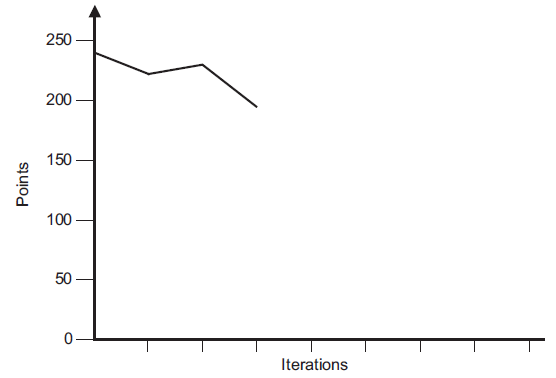
\includegraphics[scale=0.6]{burndown-real}
  \end{center}
\end{figure}

A importância do burndown chart reside no fato de mostrar rapidamente as duas mais importantes informações para o acompanhamento do projeto: quanto trabalho falta e qual é a taxa de progresso da equipe face ao decorrer do tempo e às mudanças no plano. Isto torna possível fazer previsões: no exemplo da Figura \ref{burndown-real}, pode-se estimar que o release não será concluído dentro das 8 iterações inicialmente estabelecidas.


\subsection{Um burndown bar chart do release}

O burndown chart não é capaz de reconhecer separadamente mudanças na velocidade e no escopo do projeto. Para isto foi criado o burndown bar chart.

\begin{figure}
  \caption{Separando os impactos das mudanças na velocidade e no escopo}
  \label{burndown-bar-chart}
  \begin{center}
  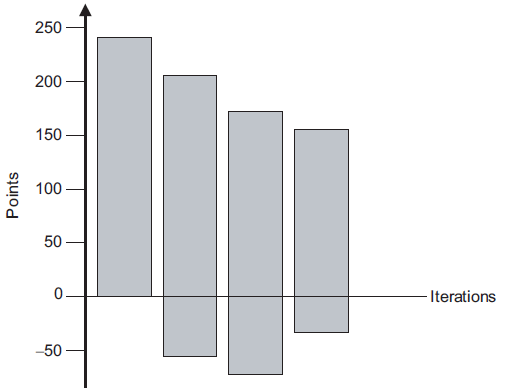
\includegraphics[scale=0.6]{burndown-bar-chart}
  \end{center}
\end{figure}

Cada barra na Figura \ref{burndown-bar-chart} representa a quantidade de esforço a ser realizado no release no momento do início de cada iteração. A parte de baixo da barra aumenta para baixo sempre que trabalho é adicionado ao projeto. A parte de baixo é diminui para cima sempre que trabalho é removido da iteração. Se a parte de baixo da barra está em um patamar inferior a zero, significa que trabalho foi adicionado ao release após o seu início.

Tome-se a Figura \ref{burndown-bar-chart} como exemplo. No início da primeira iteração, a quantidade de trabalho necessária é de 240 pontos, representada por uma barra de 0 a 240. Como no exemplo anterior, a equipe espera implementar 240 pontos em 8 iterações. Na primeira iteração, a equipe alcança a velocidade esperada, de modo que a segunda barra vai de 0 a 210 pontos. Contudo, o product owner incluiu 50 pontos no release, o que resultou em um incremento na parte de baixo da barra para o início da segunda iteração, que vai de -50 a 210. 

Cada barra é desenhada antes do início de cada iteração, com os dados referentes ao resultado da iteração anterior.

Ao fim da segunda iteração, há algumas informações interessantes:
\begin{itemize}
 \item a velocidade da equipe foi a esperada e o topo das três primeiras barras diminuiu 30 pontos cada uma;
 \item uma grande quantidade de trabalho foi adicionada, como se pode ver na parte inferior da segunda e terceira barras;
 \item ao fim da primeira iteração há mais trabalho a ser feito do que no início dela. Isto é um fator para se estar atento devido ao impacto nas estimativas do release.
\end{itemize}

Há claramente mais expressividade no burndown de barras do que no padrão. A desvantagem é que seu significado não é óbvio à primeira vista.

Olhando para o resultado da terceira iteração (4ª barra da Figura \ref{burndown-bar-chart}), percebe-se que a velocidade caiu para 20 pontos por iteração. Ainda durante a terceira iteração, o product owner retirou funcionalidades do release, o que fez a parte de baixo da barra subir na proporção do esforço removido. Contudo, no geral, ainda foi incluído mais esforço do que excluído, o que é demonstrado pela barra ainda estar abaixo de 0.

Assim, temos 4 regras simples para o burndown de barras:
\begin{enumerate}
 \item toda vez que trabalho é completado, a topo da barra desce;
 \item quando trabalho é reestimado, o topo da barra desce ou sobe, dependendo da reestimativa ser um aumento ou uma diminuição;
 \item quando trabalho é adicionado ao release, a parte de baixo da barra desce;
 \item quando trabalho é removido do release, a parte de baixo sobe.
\end{enumerate}

\begin{figure}
  \caption{Removendo trabalho de um release}
  \label{burndown-bar-chart-real}
  \begin{center}
  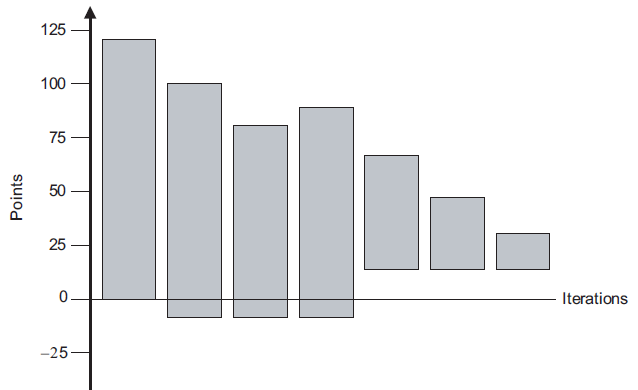
\includegraphics[scale=0.6]{burndown-bar-chart-real}
  \end{center}
\end{figure}


A Figura \ref{burndown-bar-chart-real} mostra um burndown bar chart de um projeto real. Neste exemplo, a equipe fez um bom progresso nas duas primeiras iterações. O product owner diagnosticou a necessidade de adicionar uma pequena quantidade de trabalho durante a segunda iteração. Durante a terceira iteração, a equipe descobriu que alguams de suas histórias estavam subestimadas e eles as reestimaram para cima, o que aumentou o topo da quarta barra. Antes do início da quarta iteração, o product owner removeu trabalho do plano do release, o que resultou na parte de baixo da barra ficando acima do zero, o que significa que mais trabalho foi removido pelo product owner do que adicionado por ele após o início do release. A partir daí, o projeto continuou com progresso consistente até o fim.


\section{O gráfico do estacionamento}

O gráfico do estacionamento contém uma caixa retangular para cada tema ou conjunto de user stories relacionadas dentro de um release, conforme a Figura \ref{grafico-do-estacionamento}.

\begin{figure}
  \caption{Gráfico do estacionamento mostrando quanto de cada tema foi realizado}
  \label{grafico-do-estacionamento}
  \begin{center}
  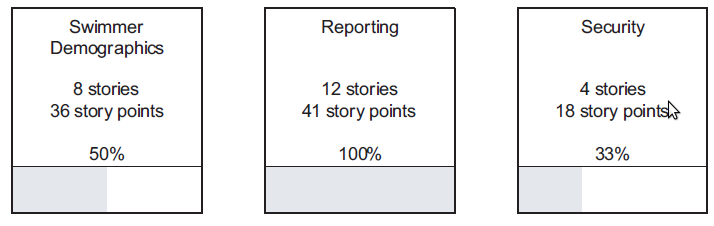
\includegraphics[scale=0.6]{grafico-do-estacionamento}
  \end{center}
\end{figure}

Cada caixa contém o nome do tema, o número de histórias, a soma das estimativas das histórias e a porcentagem de pontos terminados (vale lembrar que são considerados apenas pontos de histórias completas). Pode-se usar cores para sinalizar temas completados ou outras sinalizações específicas.


\chapter{Monitorando o plano da iteração}

Além do release, é necessário monitorar também a iteração. Veremos duas ferramentas para isto: quadro de tarefas e burndown charts.

\section{Quadro de tarefas}

O quadro de tarefas serve para organizar e dar visibilidade ao trabalho da equipe. Um exemplo é mostrado na Figura \ref{quadro-de-tarefas}.

\begin{figure}
  \caption{Quadro de tarefas}
  \label{quadro-de-tarefas}
  \begin{center}
  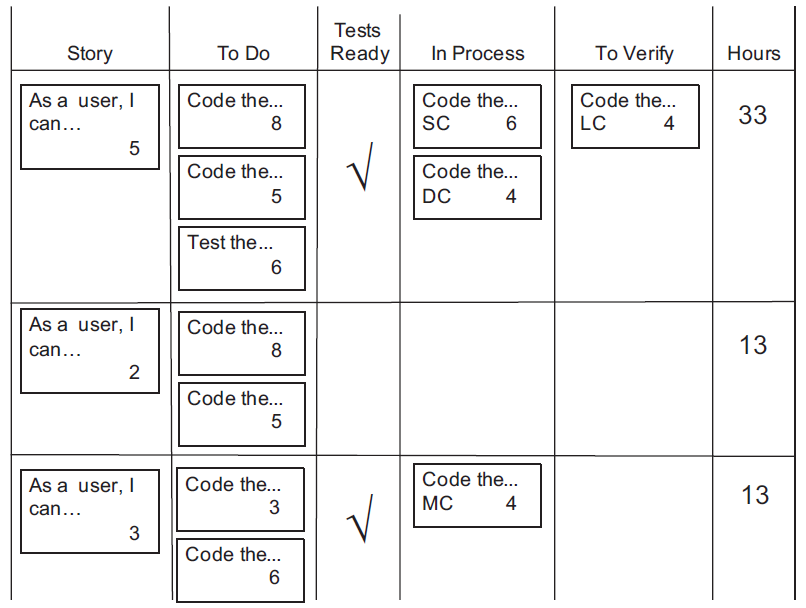
\includegraphics[scale=0.6]{quadro-de-tarefas}
  \end{center}
\end{figure}

O quadro de tarefas deve possuir uma linha para cada tarefa a ser desempenhada na iteração.  A primeira coluna contém as histórias. Uma vez que a estimativa é escrita na história, esta informação ficará visível.

A segunda coluna, ``To Do'', contém os cartões com as tarefas para cada história.

A terceira coluna, ``Tests Ready'' deve sinalizar se os testes de aceitação já foram escritos para esta história. Esta coluna é opcional, mas indicada a equipes que ainda estão iniciando em TDD.

A quarta coluna, ``In Process'', indica que a tarefa está sendo trabalhada naquele momento. Cada desenvolvedor não deve ficar alocado a mais que uma ou duas tarefas em um dado momento. Um desenvolvedor só é vinculado a uma história quando a retira da coluna ``To Do'' e a coloca em ``In Process''. É comum que esta coluna seja mais estreita, uma vez que apenas poucas tarefas estarão sendo implementadas ao mesmo tempo.

A quinta coluna, ``To Verify'', serve para que a finalização da história seja validada por alguém\footnote{Nota de Rodrigo: algumas equipes costumam mover as tarefas para ``Finalizadas'' somente no stand-up meeting, então esta coluna poderiam ficar as histórias finalizadas mas ainda não apresentadas à equipe.}. Esta coluna é opcional.

A sexta coluna, ``Hours'', traz a soma das horas das tarefas restantes, fornecendo uma clara idéia de quanto ainda falta para terminar a história. Deve ser atualizada diariamente, uma vez que os desenvolvedores podem alterar a qualquer momento as estimativas das tarefas.

Opcionalmente, pode-se utilizar uma coluna ``Done'' para as tarefas terminadas.


\section{Burndown chart da iteração}

Dependendo do tamanho das iterações, pode ser útil criar um burndown chart também para a iteração. Para iterações de uma semana, provavelmente não será necessário, sendo fundamentais para iterações de 2 semanas ou mais. A Figura \ref{burndown-chart-da-iteracao} traz um exemplo.

\begin{figure}
  \caption{Burndown chart da iteração}
  \label{burndown-chart-da-iteracao}
  \begin{center}
  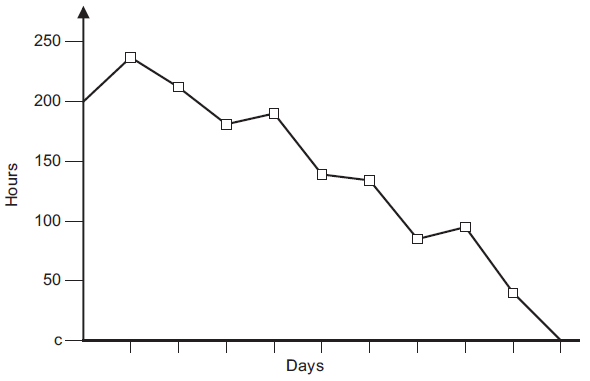
\includegraphics[scale=0.6]{burndown-chart-da-iteracao}
  \end{center}
\end{figure}

Os eixos do burndown chart da iteração são medidos em horas ideais x dias.


\section{Acompanhando o esforço gasto}

Esforço gasto não necessariamente representa progresso no projeto. É muito mais útil saber quanto falta para terminar do que quanto já foi feito. Comparações entre esforço estimado e esforço gasto deve ser feita com cuidado para não gerar pressões sobre a equipe, cujo resultado é apenas criar uma ansiedade que piora a qualidade das estimativas. Além disto, é importante ter em mente a variabilidade que é inevitável no desenvolvimento de software.


\section{Velocidade individual}

Não meça velocidades individualmente. Medições individuais de velocidade podem levar a comportamentos destrutivos para o projeto como um todo. Imagine que seja anunciado que as velocidades passarão a ser medidas individualmente iteração a iteração. Se o desenvolvedor for forçado a escolher entre terminar uma história que irá melhorar sua velocidade e ajudar alguém, o que qualquer um escolheria? 

Uma equipe ágil deve atuar como uma equipe. Valores individuais de velocidade são irrelevantes.

\end{document}
